% --------------------------------------------------------------------------
% Шаблон презентации в стилистике Университета ИТМО
% Версия шаблона 2.1. Также шаблон доступен на сайтах:
% https://www.overleaf.com/read/rpkkfchcnbsc
% https://www.overleaf.com/latex/templates/itmo-beamer-theme/fpttrgnmqwsb
% https://github.com/AlexZabashta/ITMO-Beamer-theme
% --------------------------------------------------------------------------

% Внимание!!!
% Этот документ создан для примера использования beamer стиливика.
% Не стоит воспринимать его как урок Latex или beamer!
% Ознакомьтесь с возможностями Latex и beamer (хотя бы базовыми) отдельно.


\documentclass[aspectratio=169]{beamer}
\usepackage{MIPTtheme}
% Для оформления библиографии
% \usepackage{mipt-thesis-biblatex}
% Без этой команды он иногда ругается.
\hypersetup{unicode=true}

% Пакет для "русификации" Latex.
\usepackage[english,russian]{babel}

% Чтобы адекватно работало копирование текста из полученной .pdf-ки.
\usepackage{cmap}


% Это нужно, чтобы он называл рисунки без сокращения "рис.".
% Таблицы он называет без сокращения по умолчанию.
\addto\captionrussian{\renewcommand{\figurename}{Рисунок}}

% Пакет для использования запятой в качестве десятичного разделителя.
% Следите, чтобы в формулах запятые стояли с пробелами, там где они запятые. Например $v = (x, y, z)$
\usepackage{icomma}
%\usepackage{enumitem}



% Это единственный пакет для библиографии, который у меня заработал с \footcite шаблоном.
% В презентациях лучше делать её руками через \footnote!
\usepackage[style=mla]{biblatex}
\addbibresource{diploma.bib}


% Рисунок для титульного слайда.
% \titlegraphic{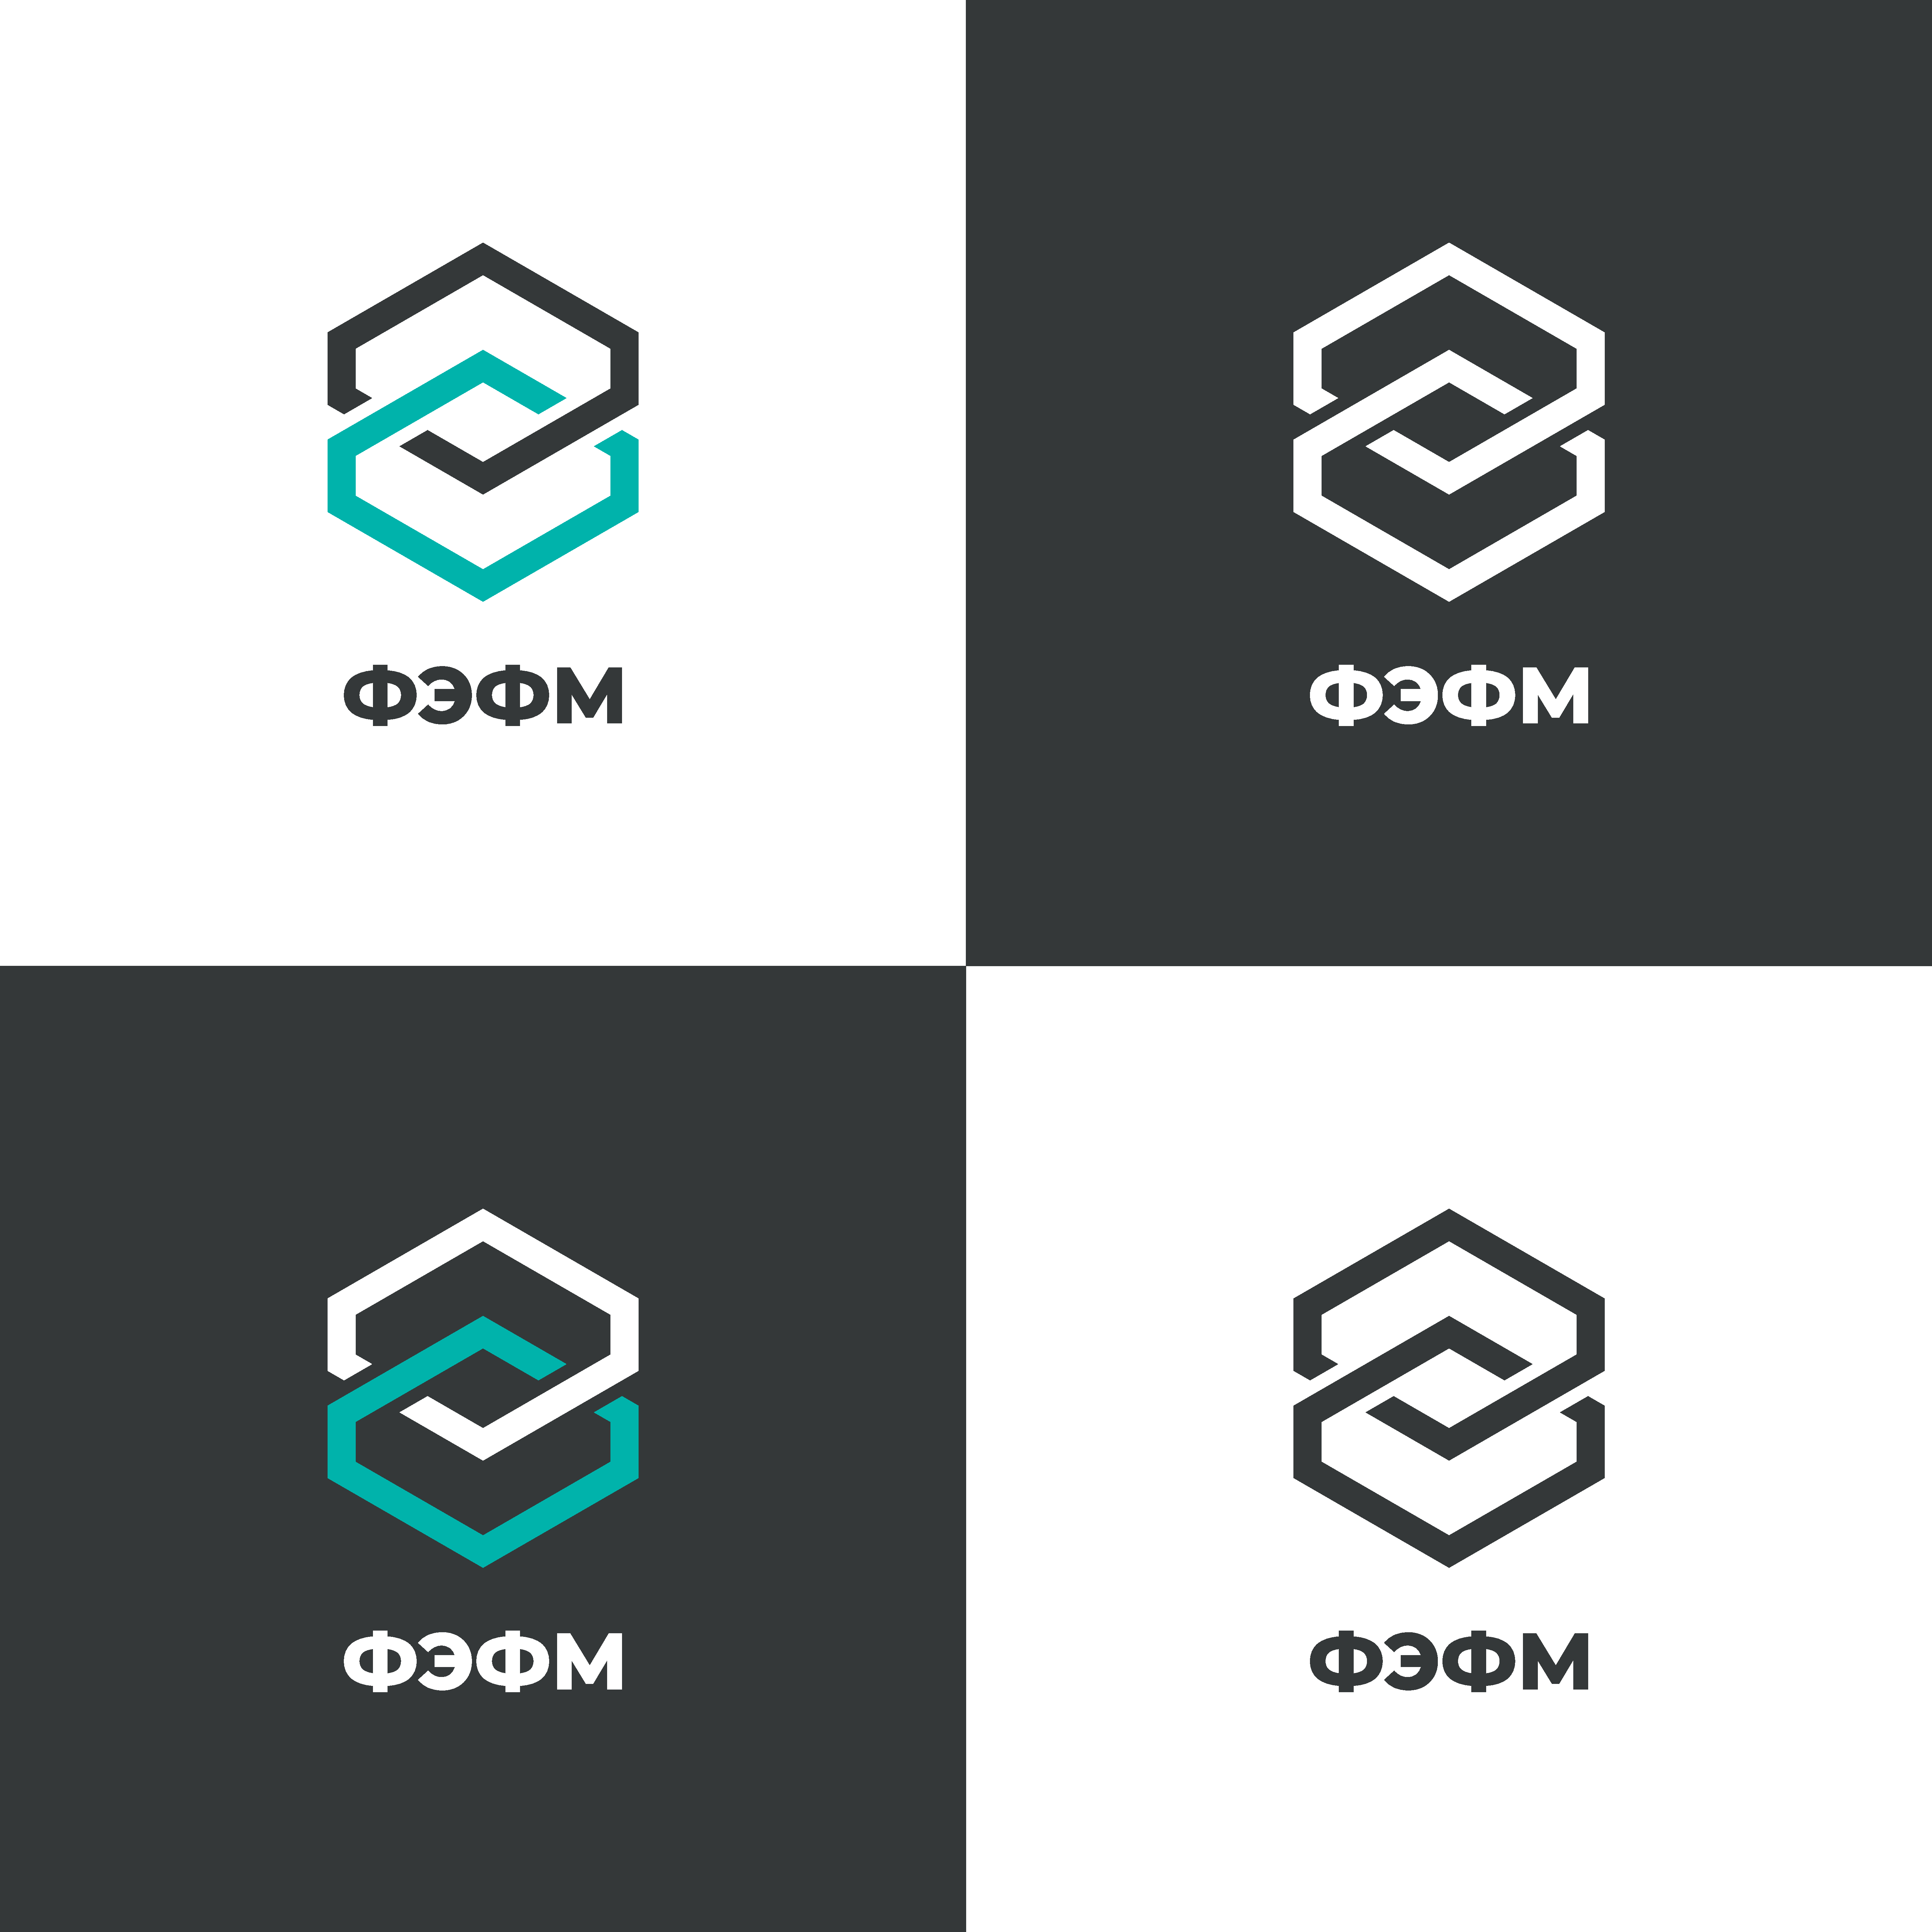
\includegraphics[scale=.8]{mipt/Логотип_ФЭФМ_макет.pdf}}

% Логотип внизу каждого слайда
% \logo{
\includegraphics[height=0.5cm]{mipt/mipt_rus_text_eps.pdf}}


% Поля title, author, subject, keywords используются при формировании pdf документа.
% Поэтому их нужно заполнять, даже если вы формируете титульный слайд руками.

% Формат: \title[Короткое название]{Полное название}
\title[MIPT LaTeX]{Механические и оптические свойства изготовленных двухфотонной нанолитографией 3D-структур, изученные при помощи наноиндентирования и оптических методов}

%\subtitle[short subtitle]{long subtitle}
% В квадратных скобках короткая запись авторов.
\author[Щербаков Д.А.]{Щербаков Денис Алексеевич}
\supervisior{д.ф.~-~м.н., профессор Витухновский Алексей Григорьевич}
\department{Физтех-школа электроники, фотоники и молекулярной физики}
\institute[МФТИ]{Московский физико-технический институт}
\subtitle[]{Выпускная квалификационная работа на степень магистра}
\where{г.~Москва}
\date{\today}

% Тематика и ключевые слова.
\subject{Beamer template}
\keywords{ITMO University, LaTex teamplate, beamer}


% По умолчанию внизу каждого слайда пишется название презентации (\inserttitle).
% Этот текст можно заменить на другой, например:
\setfootlinetext{\insertsection}


\begin{document}

% [plain] - модификатор для создания пустого слайда (без нижней полосы).
% Идеально подходит для создания первого (титульного) и последнего слайда с полигональным фоном,
% либо для переходных слайдов между главами или слайдов с оглавлением.

% \titlepage - команда для автоматической генерации контента титульного слайда.
\begin{frame}[plain]
    \titlepage
\end{frame}


% \miptpolygons - команда для создания полигонального фона.
% Используется для создания фона на первом (титульном) и последнем слайде.


% Если вас не устраивает контент стандартного титульного слайда,
% то можете сами его скомпоновать, либо исправить .sty файл.


% \begin{frame}[plain]
% 	\miptpolygons{
% 	\begin{minipage}{0.2\paperwidth}
% 	    \begin{flushleft}
% 	    
\includegraphics[height=0.15\paperheight]{mipt/image3_pattern.png}
% 	    \end{flushleft}
% 	\end{minipage}
% 	\hfill
% 	\begin{minipage}{0.2\paperwidth}
% 	    \begin{flushright}
% 	    	    
\includegraphics[height=0.15\paperheight]{mipt/image2_pattern.png}
% 	    \end{flushright}
% 	\end{minipage}
% 	\vfill
% 		{\Large \textbf \inserttitle} 
% 	\vfill
% 		{\textbf{Выпускная квалификационная работа магистра по специальности 03.04.01 <<Прикладные математика и физика>>}} 
% 	\vfill
% 		{\textbf \insertauthor}
% 	\vfill
% 		Научный руководитель: Витухновский А.Г., профессор, д.ф.~- м.н \par
% 		Рецензент: Фамилия И.О., звание, степень
% 	\vfill
% 		{\small \insertplace, \insertdate}
% }
% \end{frame}



% Не стоит делать оглавление в коротких презентациях.
% Переходы между главами лучше делать "руками".

% \AtBeginSection[]
% {
%     \begin{frame}[plain]
%         \frametitle{План Презентации}
%         \Large
%         \tableofcontents[currentsection]
%     \end{frame}
% }


% \begin{frame}{Footcite and Footnote}

% Пример сноски\footnote{Например её можно использовать для цитирования.}.

% \end{frame}

\section{Актуальность}

\subsection{Применение DLW -- нанолитографии}

\begin{frame}
\frametitle{Применение DLW -- нанолитографии}
\begin{columns}[c] 
\column{0.45\textwidth}{
\begin{enumerate}%[label =\alph*]
    \item Метаматериалы %\footcite{Metamaterweg}
    \item Микроробототехника %\footcite{4dmetamat}
    \item 3D волноводы %\footcite{shelby2001experimental}
    \item Фотонные кристаллы %\footcite{photcryscol}
\end{enumerate}
}
\column{0.55\textwidth}{
    \begin{minipage}[t]{0.45 \textwidth}
        \textbf{(1)} 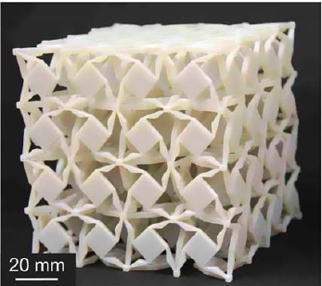
\includegraphics[width = \linewidth]{fig/3d_meta.png}
    \end{minipage}
    \hfill
    \begin{minipage}[t]{0.45 \textwidth}
        \textbf{(2)} 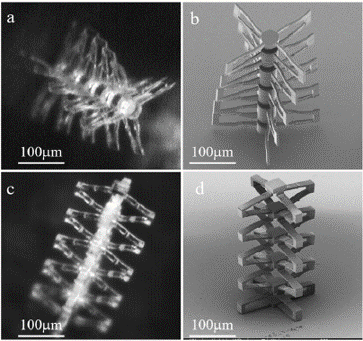
\includegraphics[width = \linewidth]{fig/4d_microrobot.png}
    \end{minipage}
    \begin{minipage}[t]{0.45 \textwidth}
        \textbf{(3)} 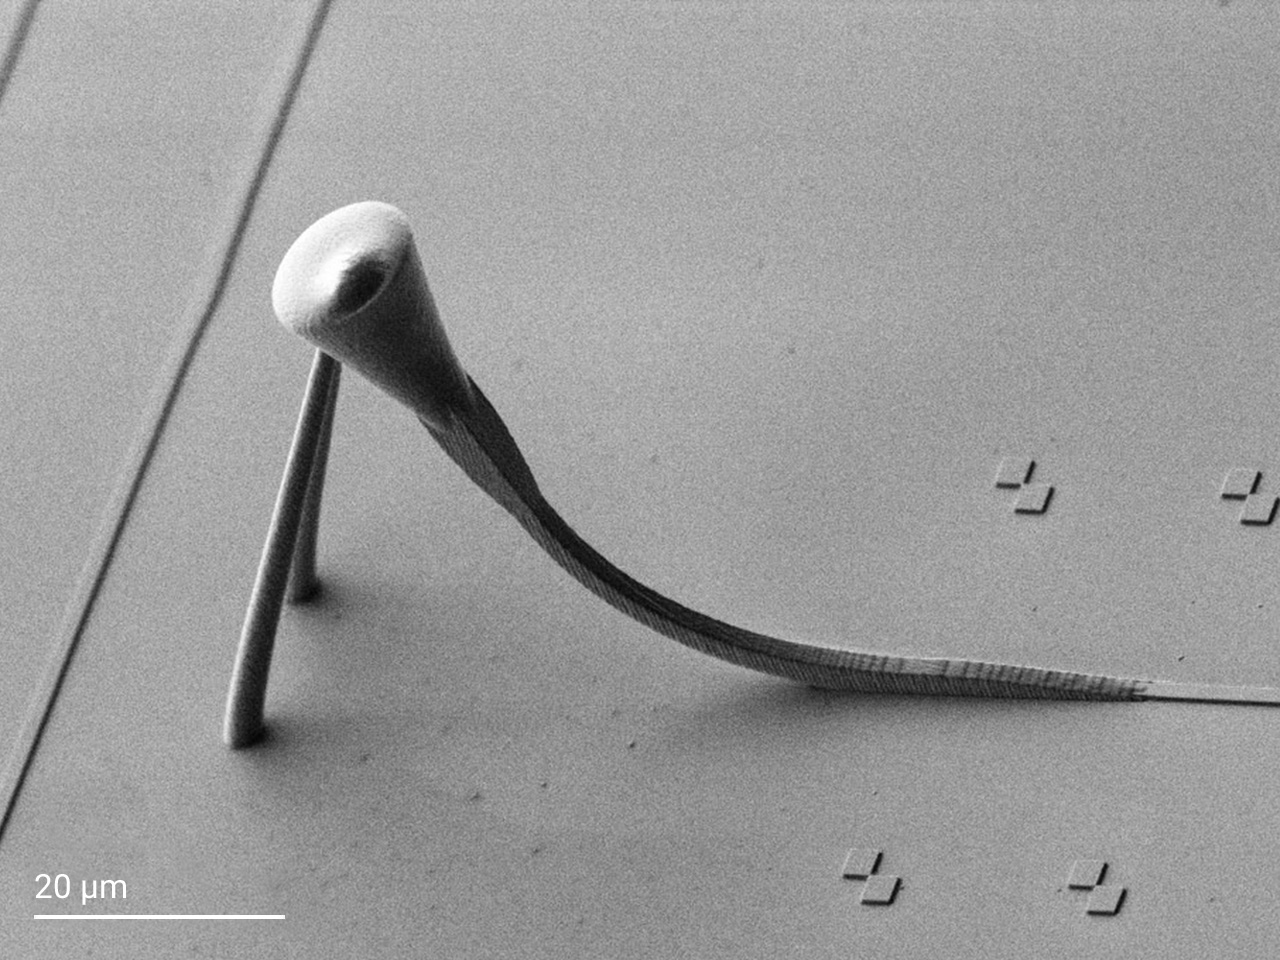
\includegraphics[width = \linewidth]{fig/Freeform-3D-fiber-to-chip-coupler-Gallery.jpg}
    \end{minipage}
    \hfill
    \begin{minipage}[t]{0.45 \textwidth}
        \textbf{(4)} 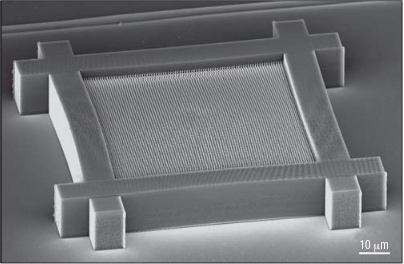
\includegraphics[width = \linewidth]{fig/Screenshot_2021-10-04 nmat1155 - 259 pdf.png}
    \end{minipage}
}
\end{columns}
\end{frame}


\subsection{Цель работы}

\begin{frame}{Цель работы}
       Поиск оптимальных параметров DLW -- нанолитографии с целью создания механически устойчивых 3D структур сложной топологии, а также структур требующие высокого разрешения литографии. В работе использовалась новый фоторезист, имеющий перспективу для DLW~--~нанолитографии благодаря своим оптическим свойствам. С этой целью проведено исследование приведенного модуля Юнга $E_r$ и степени конверсии $DC$ изготовленных 3D-микроструктур методами наноиндентирования и рамановской спектроскопии. 
\end{frame}

\section{Изготовление образцов} 

\subsection{DLW -- нанолитография}

\begin{frame}{DLW -- нанолитография}
    \begin{columns}[c]
    \column{0.35 \linewidth}
    {Ключевые факторы при изготовлении структур методом DLW:
    \begin{itemize}
        \item Скорость сканирования
        \item Мощность лазерного излучения
        \item Фотокомпозиция (мономер + фотоинициатор)
    \end{itemize}
    }
    \column{0.55 \linewidth}{
    \begin{figure}
        \hspace*{-4em}\raisebox{0em}{
        \begin{tikzpicture}
                \node (a) {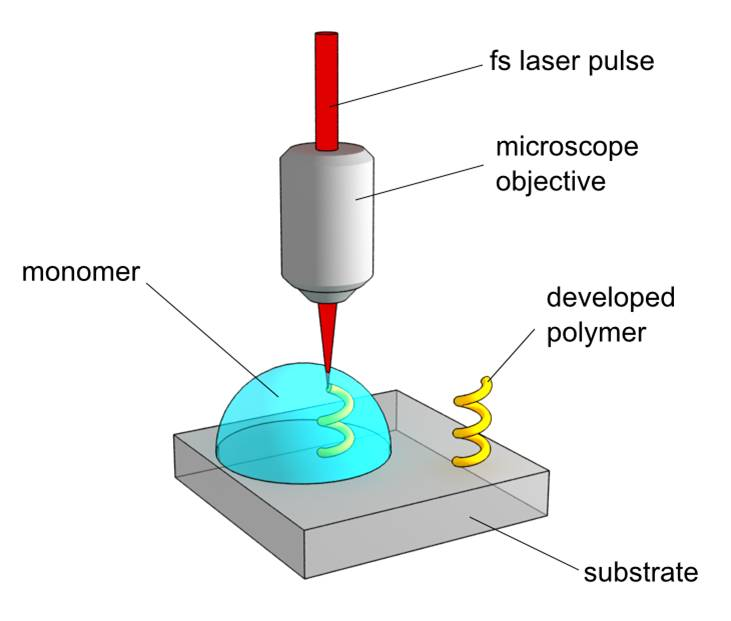
\includegraphics[trim= 0 0 0 0,clip,width = 0.75\textwidth]{fig/image1.png}};
                \node at (a.north west)[xshift=5mm,yshift=-5mm]{\textbf{(a)}};
                \node (b) at (a.right)[xshift=13mm,yshift=8mm] {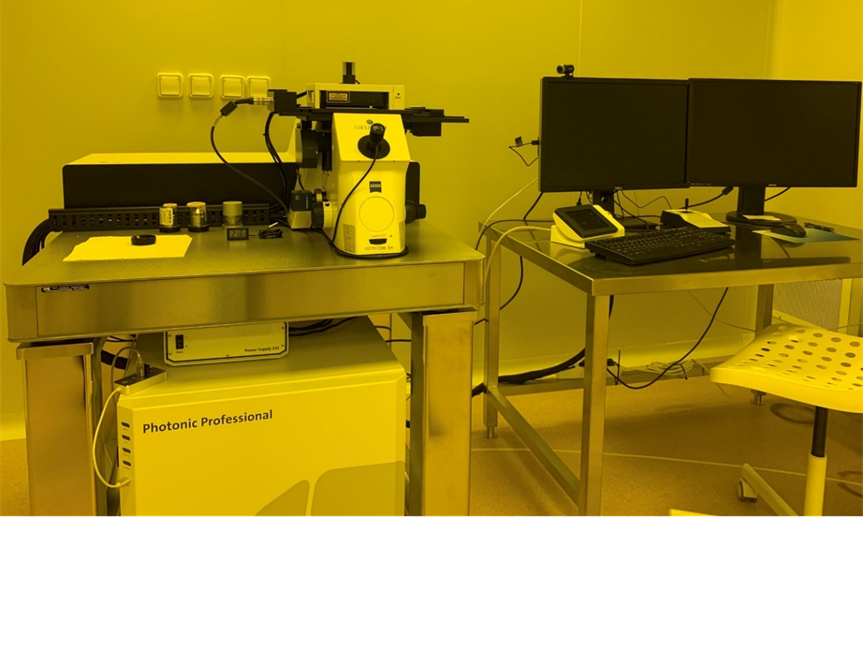
\includegraphics[trim= 0 150 300 0,clip, width = 0.45\textwidth]{fig/nanoscribe_mipt.png}};
                \node at (b.north west)[xshift=5mm,yshift=-5mm]{\textbf{(б)}};
        \end{tikzpicture}}
        \caption*{(a)~Технология Прямого Лазерного Письма (Direct~Laser~Writing~---~DLW). (б)~Нанолитограф <<Nanoscribe Professional GmbH>>}
        \label{fig:DLW}
    \end{figure}

    }
    \end{columns}
\end{frame}

% \begin{frame}{DLW -- нанолитография}

%     \begin{figure}
%         \centering
%         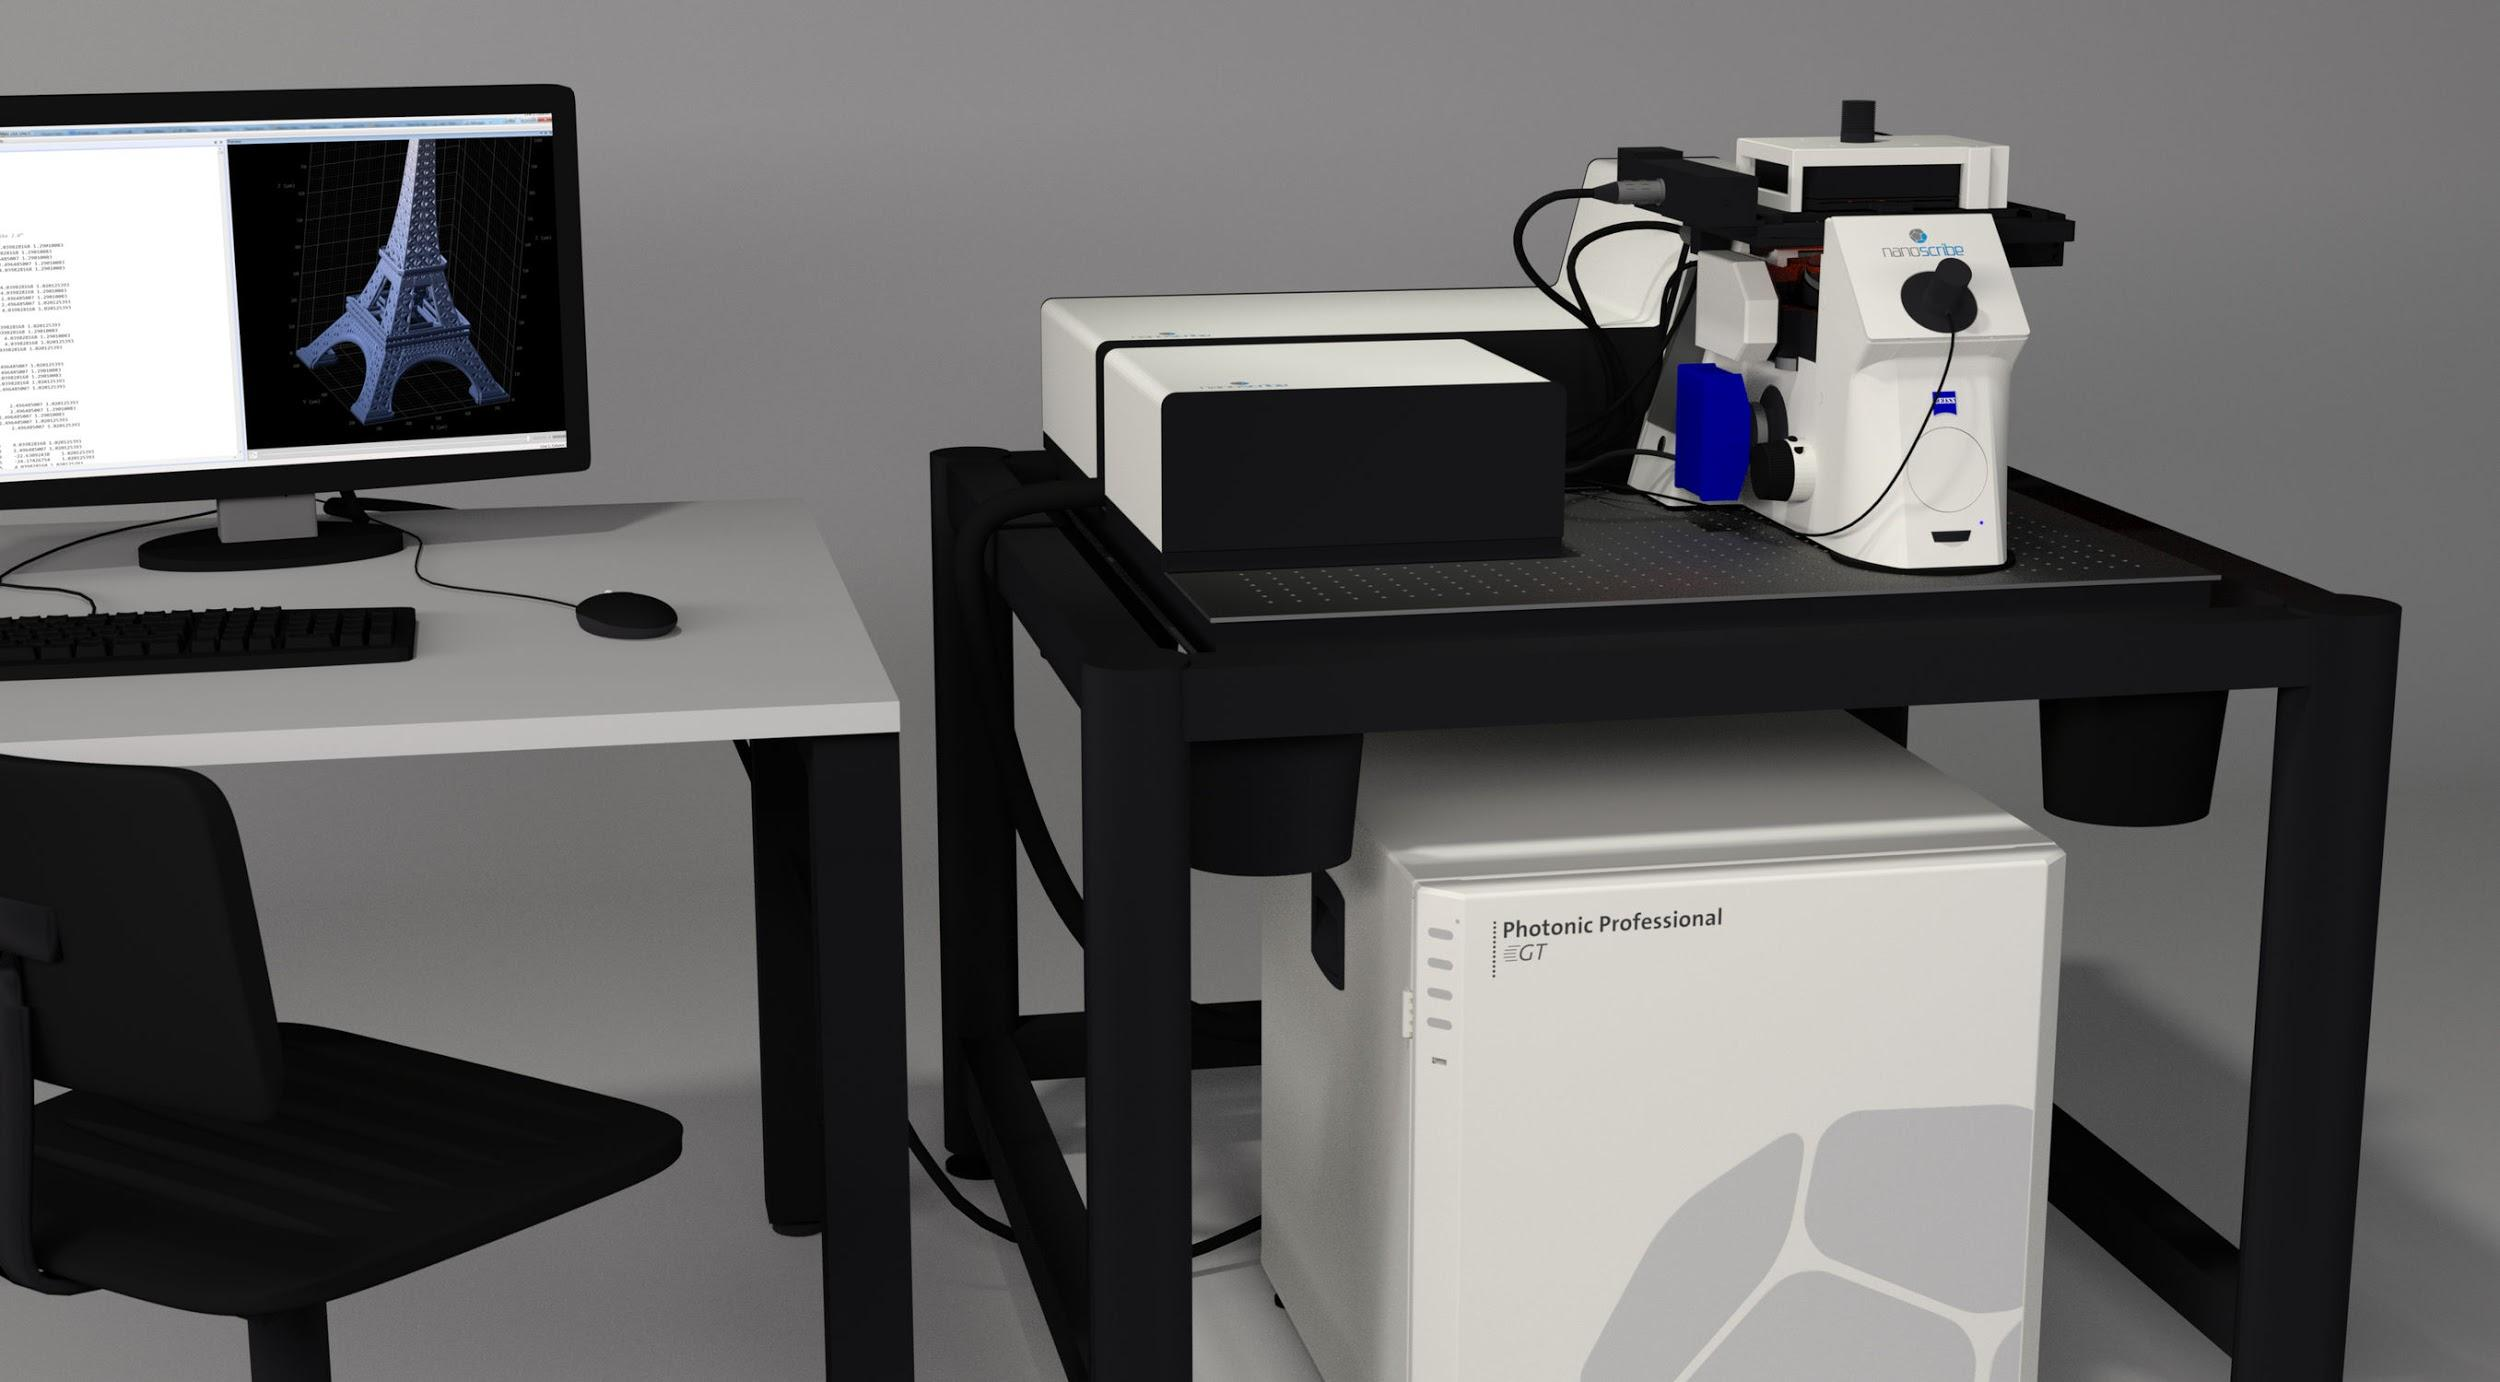
\includegraphics[width = 0.75\textwidth]{fig/image1.jpg}
%         \caption*{Нанолитограф <<Nanoscribe Professional GmbH>>}
%         \label{fig:DLW}
%     \end{figure}

% \end{frame}

\begin{frame}{DLW -- нанолитография}
    \begin{figure}
        \begin{minipage}{0.6\linewidth}
            \raggedleft
             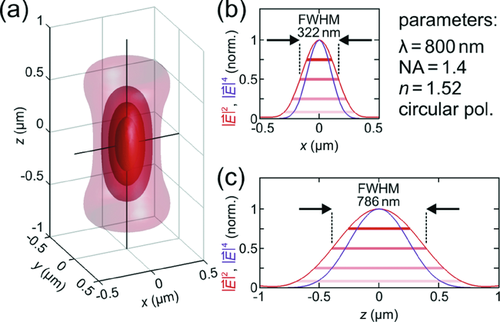
\includegraphics[height = 0.5\textheight]{fig/lpor201100046-fig-0002-m.png}  
        \end{minipage}
        \hfill
        \begin{minipage}{0.35\linewidth}
                \captionof*{figure}{(a)Пространственное распределение интенсивности гауссового пучка. (b) Распределение интенсивности поглощения вдоль оси x. (c) Распределение интенсивности поглощения вдоль аксиальной оси z. Цветами показаны случаи для одно-(красный) и двухфотонного(пурпурный) поглощения излучения.}
        \end{minipage}
        \caption*{\footcite{https://doi.org/10.1002/lpor.201100046}}
    \end{figure}
    % \begin{thebibliography}
    % \bibitem[sted]{sted}
    % Joachim Fischer and Martin Wegener, “Three-dimensional optical laser lithography beyond the diffraction", \textit{Laser & Photonics Reviews} Vol. 7, no. 1, 2013, p. 22--44.
    % \end{thebibliography}
\end{frame}

\begin{frame}{DLW -- нанолитография}
    \begin{figure}
        \begin{minipage}{0.3\linewidth}
         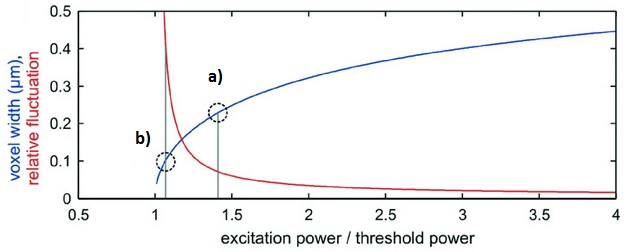
\includegraphics[width = 1\linewidth]{fig/lpor201100046-fig-0005-m_width_ (1).jpg}
        \end{minipage}
        \begin{minipage}{0.3\linewidth}
            \raggedleft
            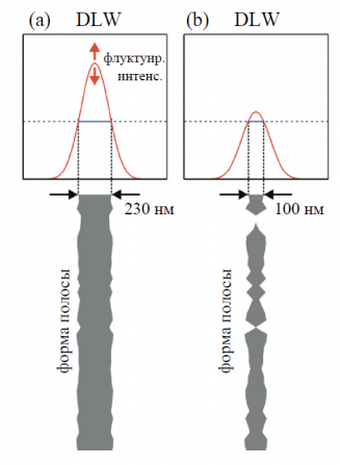
\includegraphics[height = 0.65\textheight]{fig/DLW_lines.png}
        \end{minipage}
        \hfill
        \begin{minipage}{0.35\linewidth}
            \captionof*{figure}{Флуктуация ширины линии, вызванные флуктуациями мощности лазера. (a)Рисование линии при мощности излучения в разы выше порога. Флуктуации линии порядка $\sim 7\%$. (b)Рисование линии при мощности излучения вблизи порога. Флуктуации линии порядка $\sim 42\%$.}
        \end{minipage}
        \caption*{\footcite{https://doi.org/10.1002/lpor.201100046}}
    \end{figure}
\end{frame}

\subsection{Морфология вокселя}

\begin{frame}{Морфология вокселя}
        \begin{figure}
            \begin{minipage}{\linewidth}
                \centering
                \begin{tikzpicture}
                    \node (a){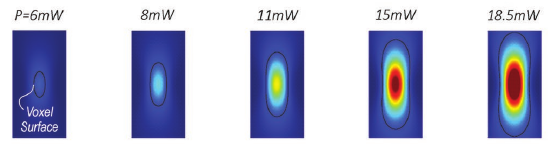
\includegraphics[width = \linewidth]{fig/image6.png}};
                \end{tikzpicture}
            \end{minipage}
            % \hfill
            % \begin{minipage}{0.49\textwidth}
            %     \begin{center}
            %         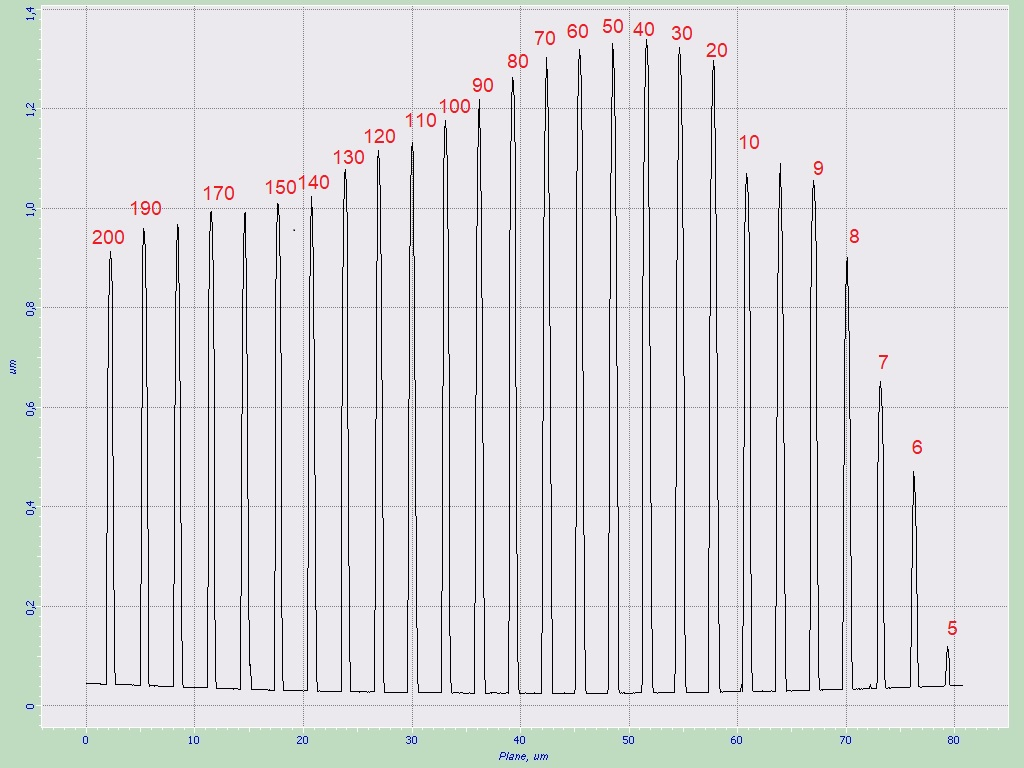
\includegraphics[width = \textwidth]{fig/image16.jpg}
            %     \end{center}
            % \end{minipage}
            \caption*{Численный расчет размера вокселя в зависимости от мощности \footcite{Mechrambald}}
        \end{figure}
\end{frame}

\begin{frame}{Морфология вокселя}
        \begin{figure}
                \begin{tikzpicture}
                    \node (b){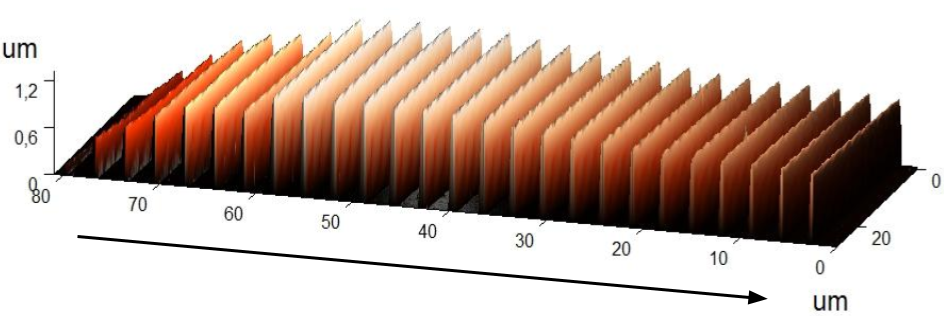
\includegraphics[width = \linewidth]{fig/3D_AFM.png}};
                    % \node at(b.north west){(б)};
                    \node at (b.south)[xshift=-5mm,yshift =0mm]{$V \uparrow (t_{exp} \downarrow)$};
                \end{tikzpicture}
            % \hfill
            % \begin{minipage}{0.49\textwidth}
            %     \begin{center}
            %         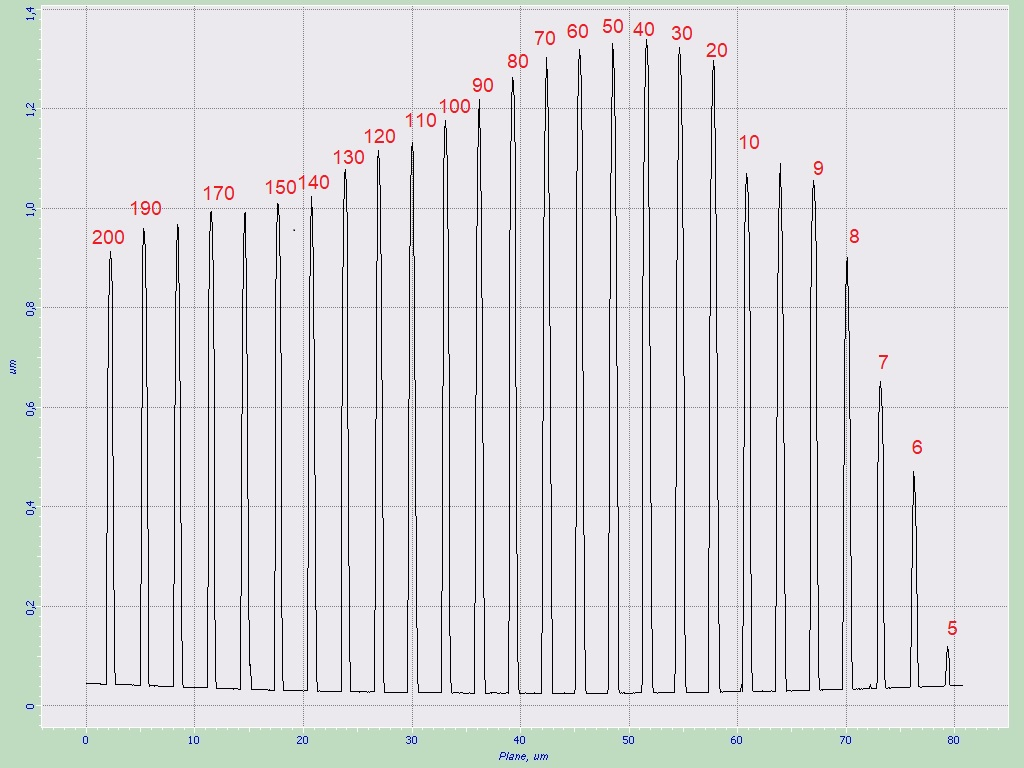
\includegraphics[width = \textwidth]{fig/image16.jpg}
            %     \end{center}
            % \end{minipage}
            \caption*{3D изображение АСМ массива линейных воксельных элементов.}
        \end{figure}
\end{frame}

\begin{frame}{Морфология вокселя}
        \begin{figure}
            % \begin{minipage}{0.4\linewidth}
            %     (\textbf{\RomanNumeralCaps{1}})~Аномальное поведение (Эффект Шварцшильда).
            %     \\
            %     (\textbf{\RomanNumeralCaps{2}})~Классическое поведение.
            % \end{minipage}
            % \hfill
            \begin{minipage}{0.55\linewidth}
                \hspace*{-3em}\raisebox{0em}{
                \begin{tikzpicture}
                    \node (h) {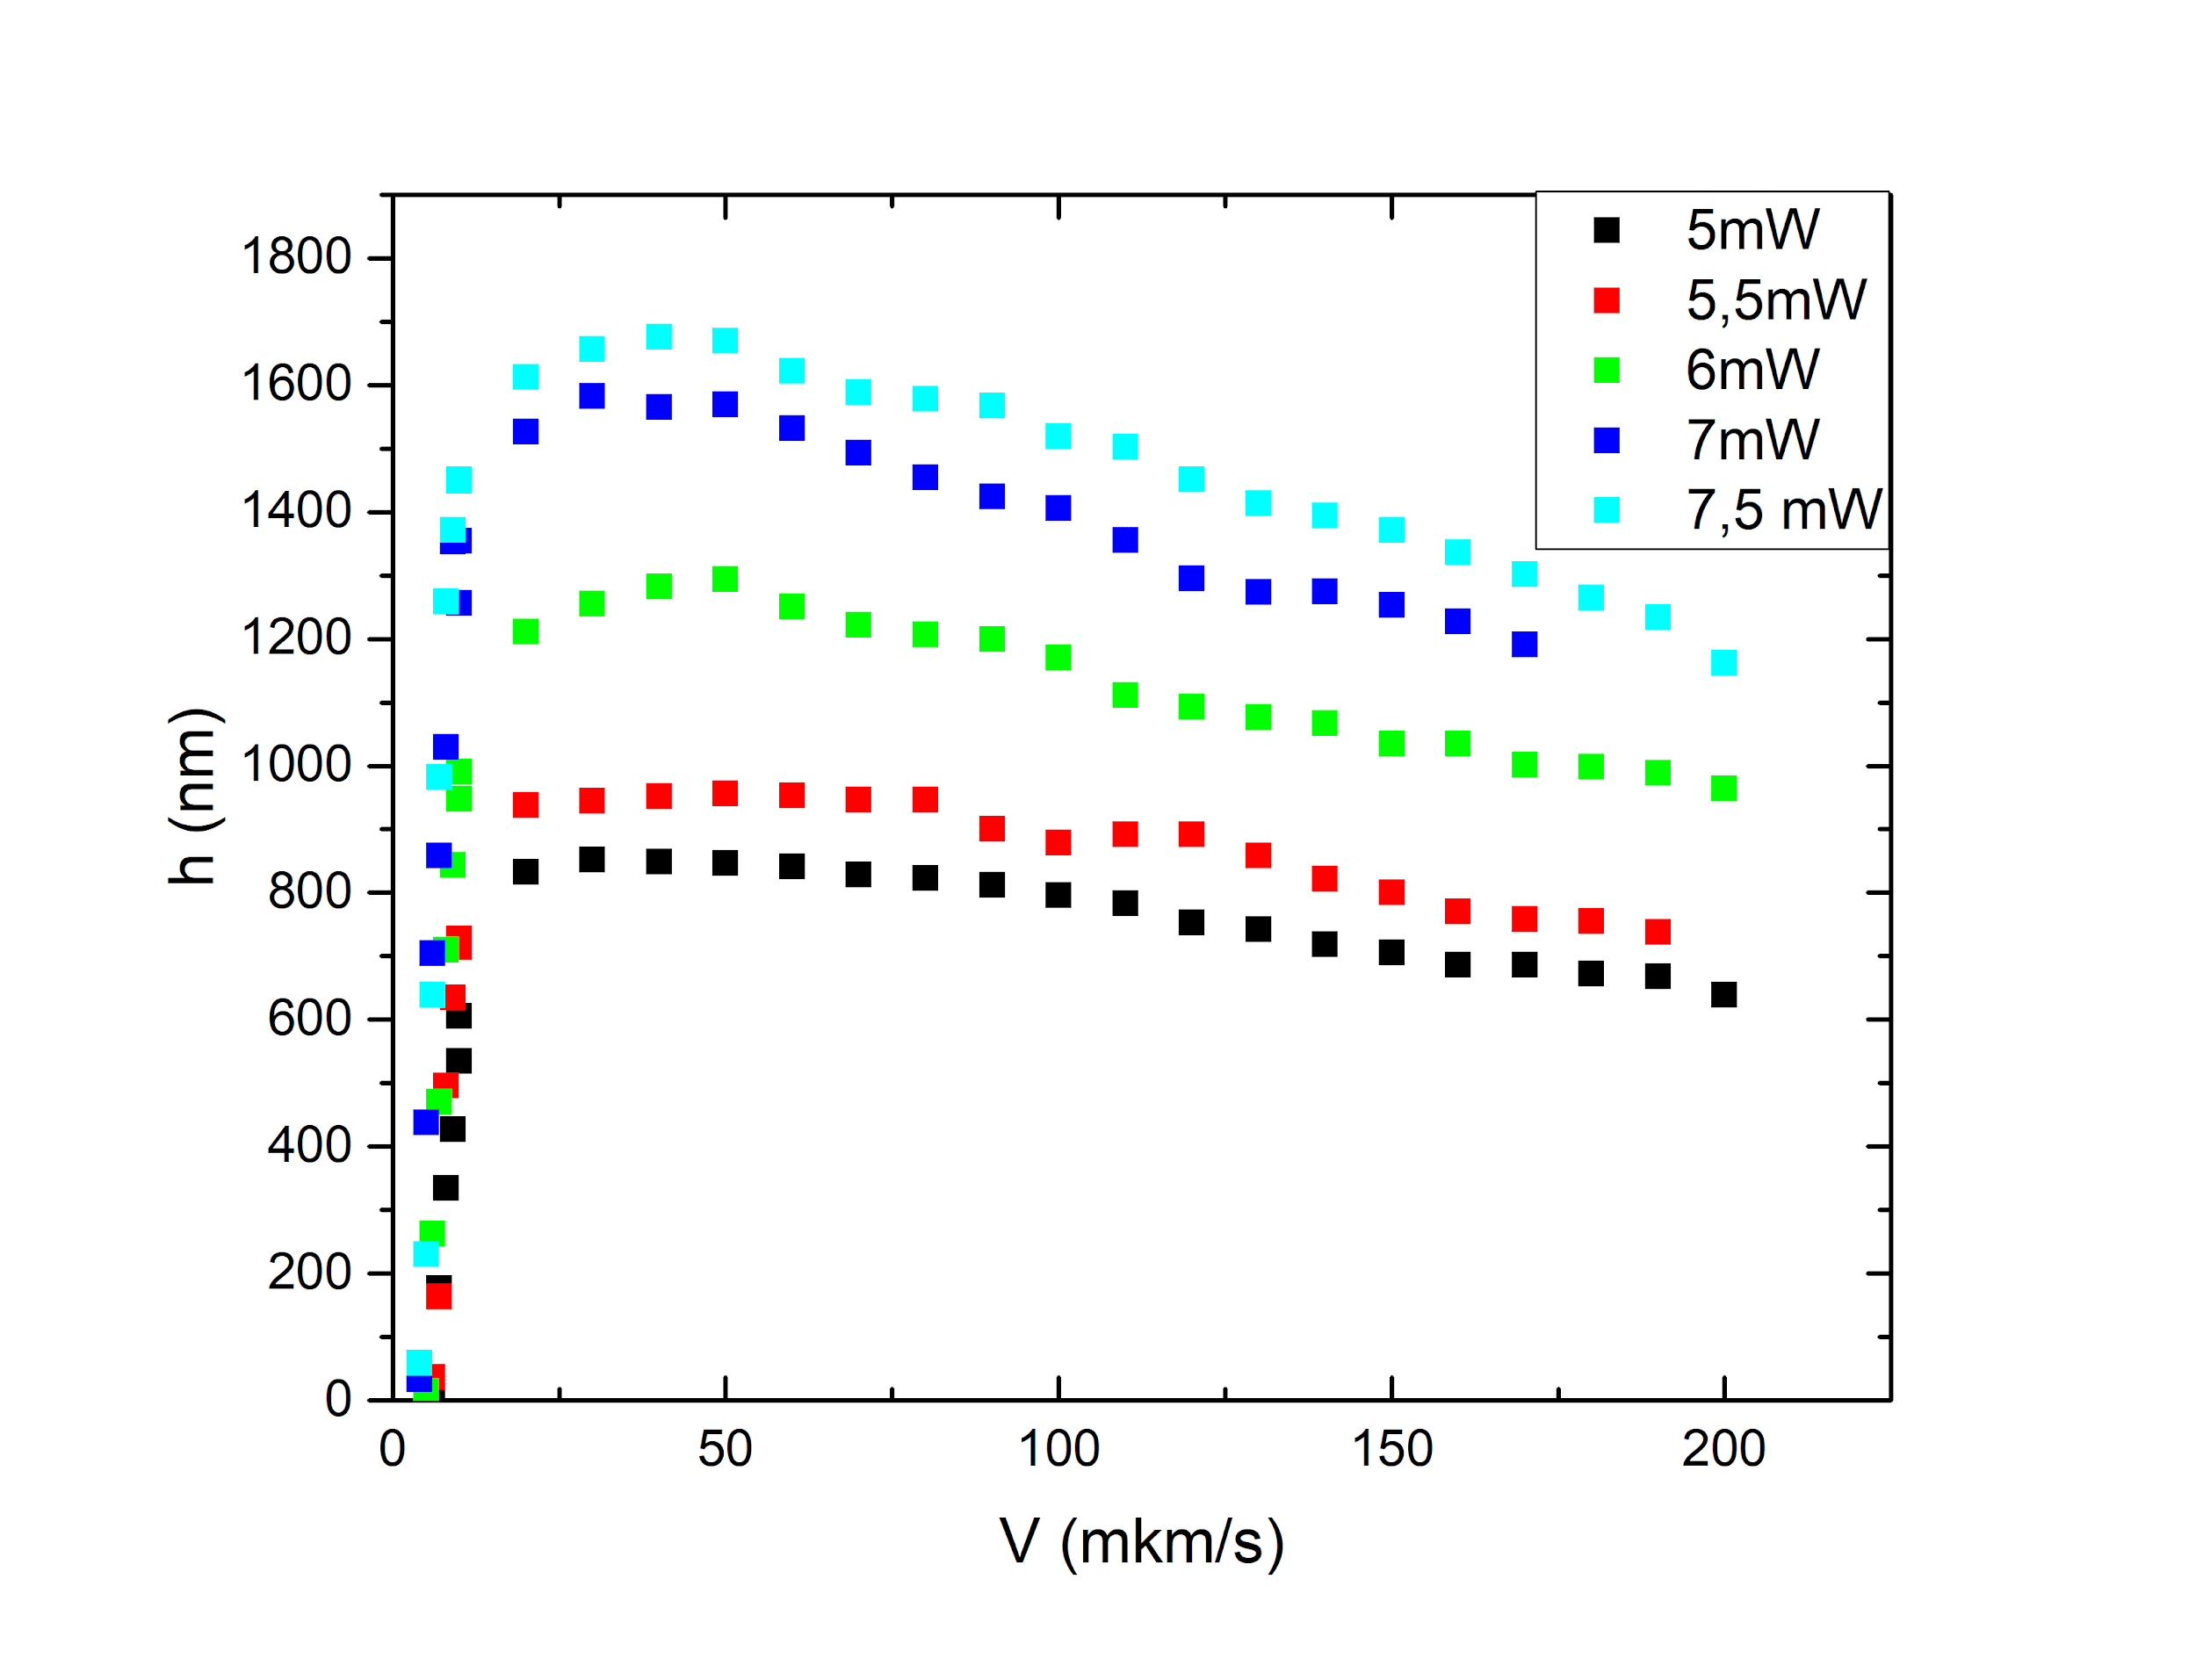
\includegraphics[trim=50 100 150 150, clip,height = 0.6\textheight]{fig/image18.png}};
                    \draw[dashed] (line) (-11mm,-18mm) -- +(0,0.6\textheight*0.81);
                    \node (I) at (h.west)[xshift=20mm,yshift=-10mm] {\Large\textbf{\RomanNumeralCaps{1}}};
                    \node (II) at (h.east)[xshift=-25mm,yshift=-10mm] {\Large\textbf{\RomanNumeralCaps{2}}};
                    % \node[left=of I]{Аномальное поведение(Эффект Шварцшильда)};
                    % \node[right= of II]{Классическое поведение};
                \end{tikzpicture}}
                \captionof*{figure}{Зависимость полувысоты вокселя от скорости сканирования. I~область~---~аномальное поведение (Эффект Шварцшильда), II~область~---~ классическое поведение}
            \end{minipage}
            \hfill
            \begin{minipage}{0.40\linewidth}
                \hspace*{-3em}\raisebox{1em}{
                \begin{tikzpicture}
                    \node (D_2) {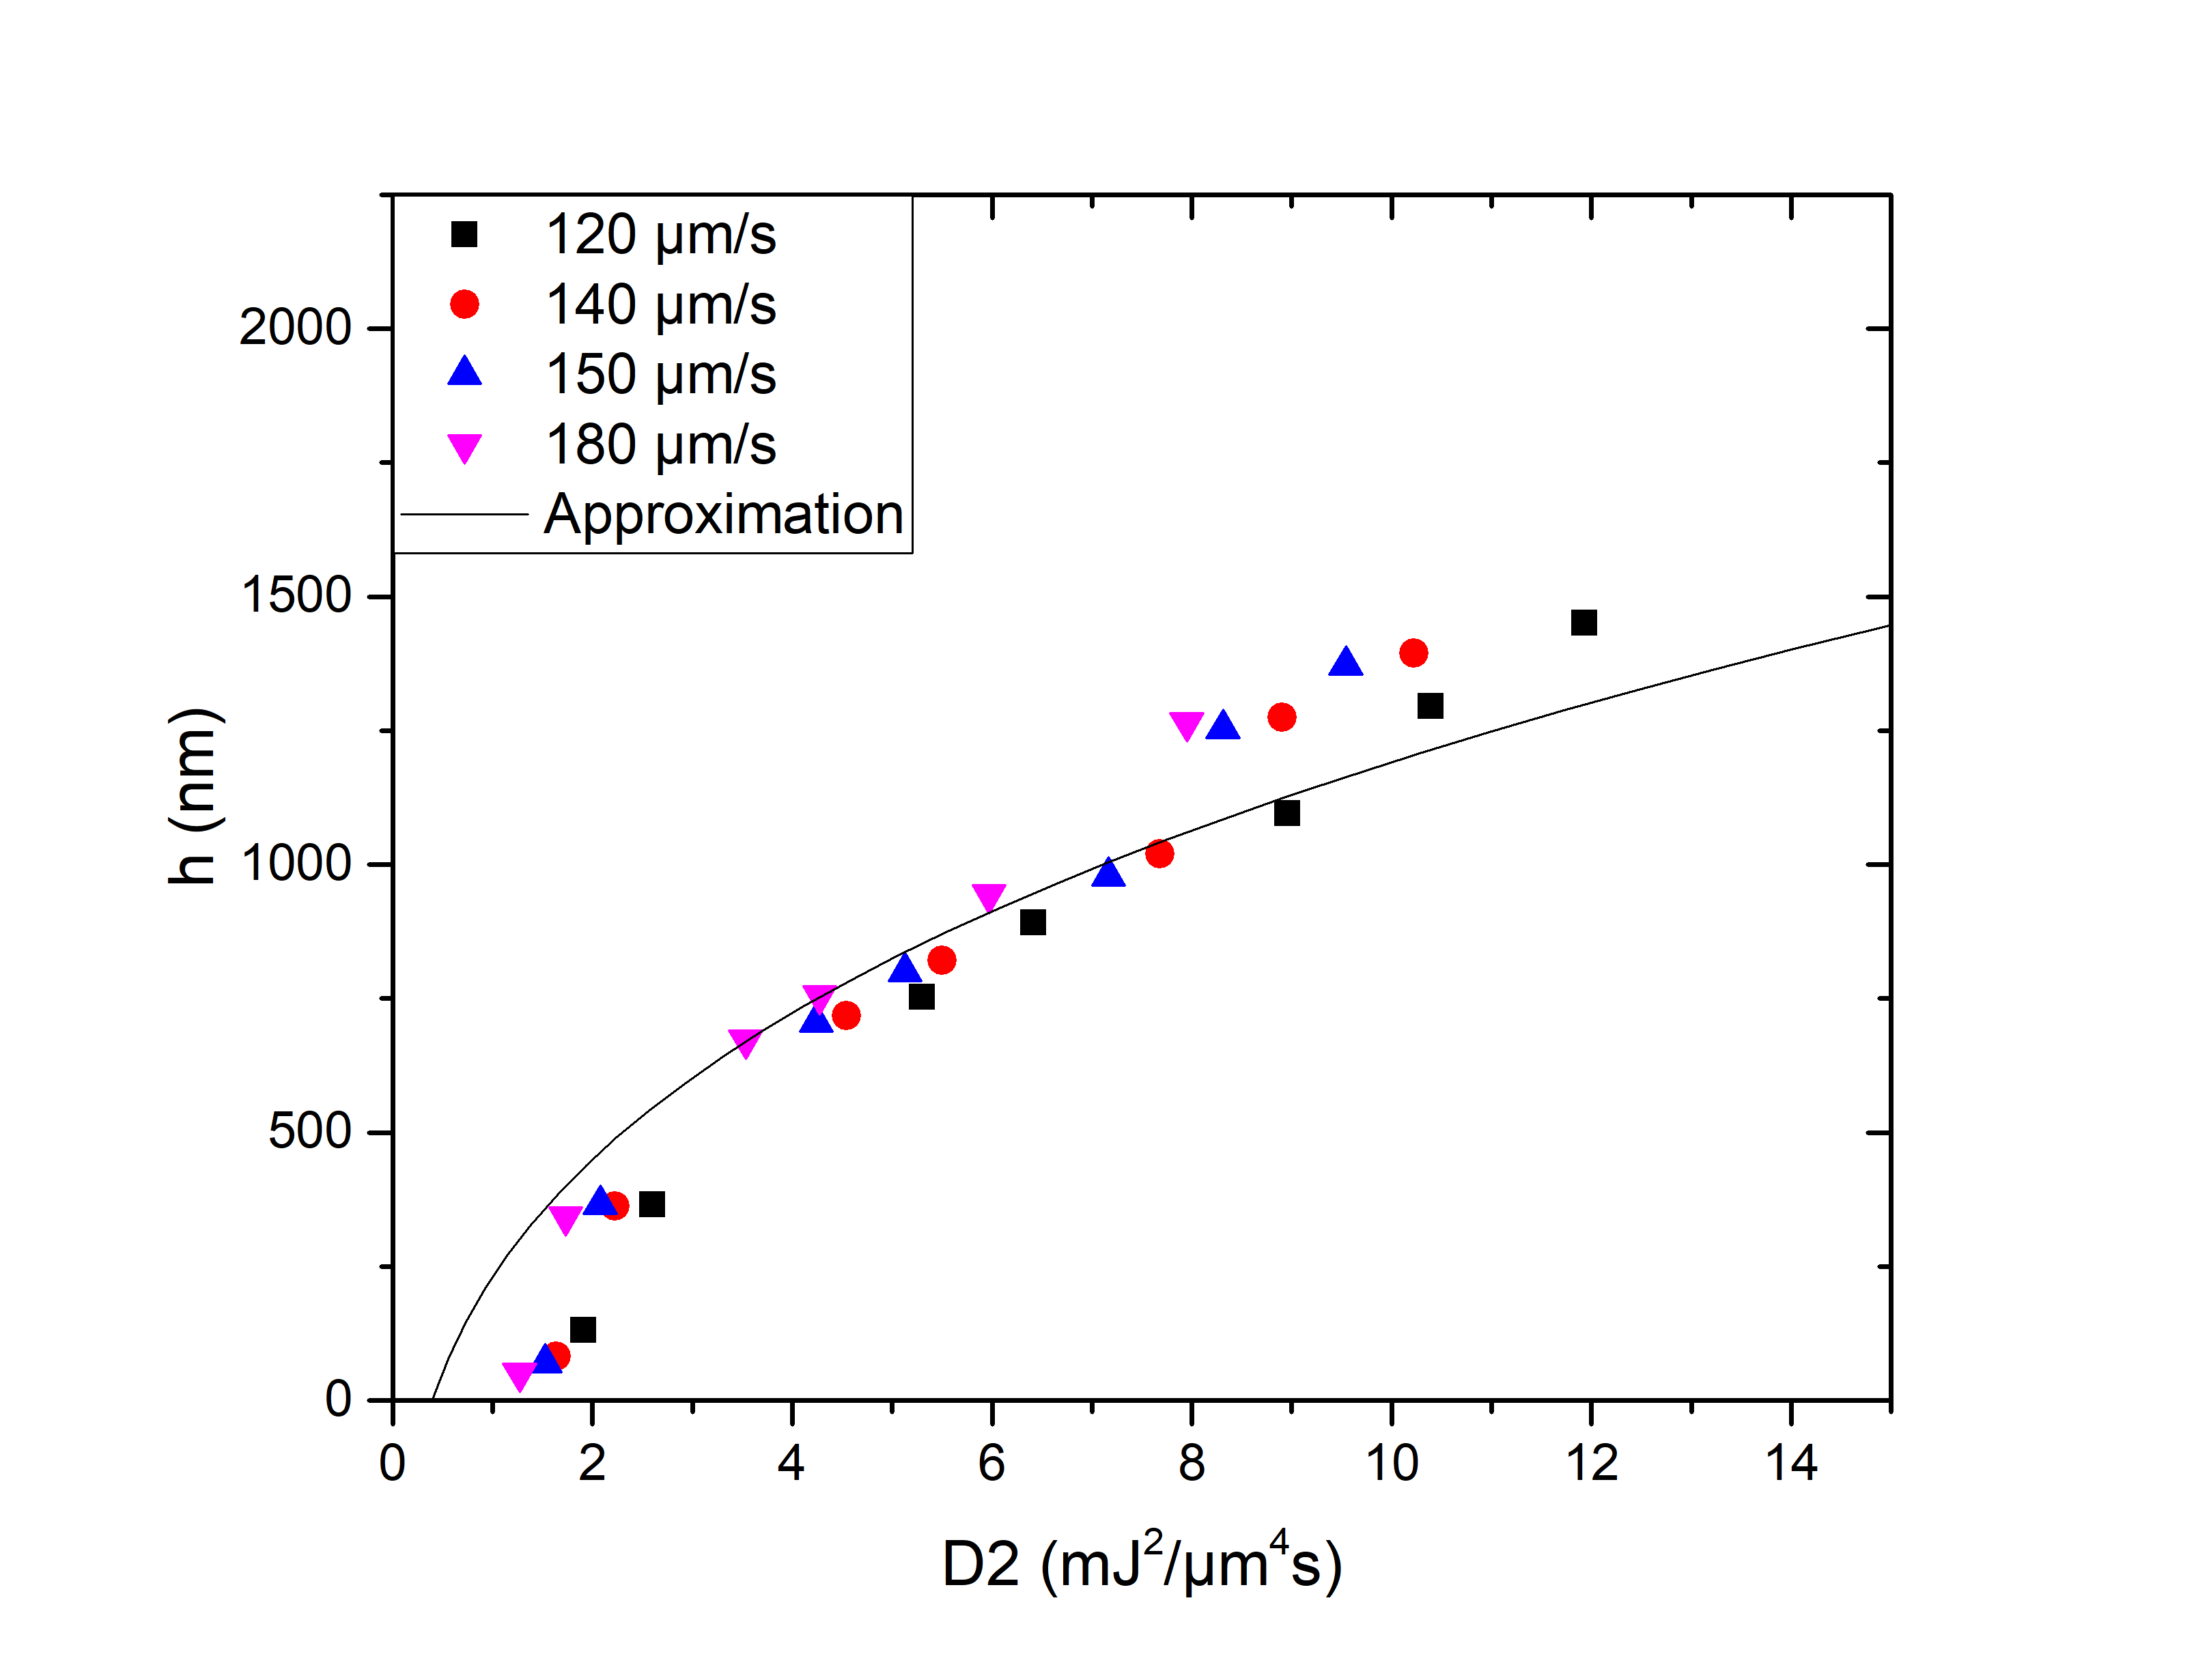
\includegraphics[trim=50 25 25 60, clip,height = 0.6\textheight]{fig/h(D2)_dz=450_Pth=0,4mW.png}};
                    \node[draw] at (D_2.north east)[xshift=-25mm, yshift=-36mm] {$D_2 = \frac{LP^2}{\updelta_{\mathrm{Abbe}}^3\, V}$};
                \end{tikzpicture}}
                \captionof*{figure}{Зависимость полувысоты вокселя от поглощенной дозы $D_2$}
            \end{minipage}
            \label{fig:h(V)_LP}
        \end{figure}
\end{frame}

\subsection{Алгоритм изготовления}

\begin{frame}{Алгоритм изготовления}
            \begin{figure}
                \begin{minipage}[t]{0.45\linewidth}
                    \textbf{(a)} \\ 
                    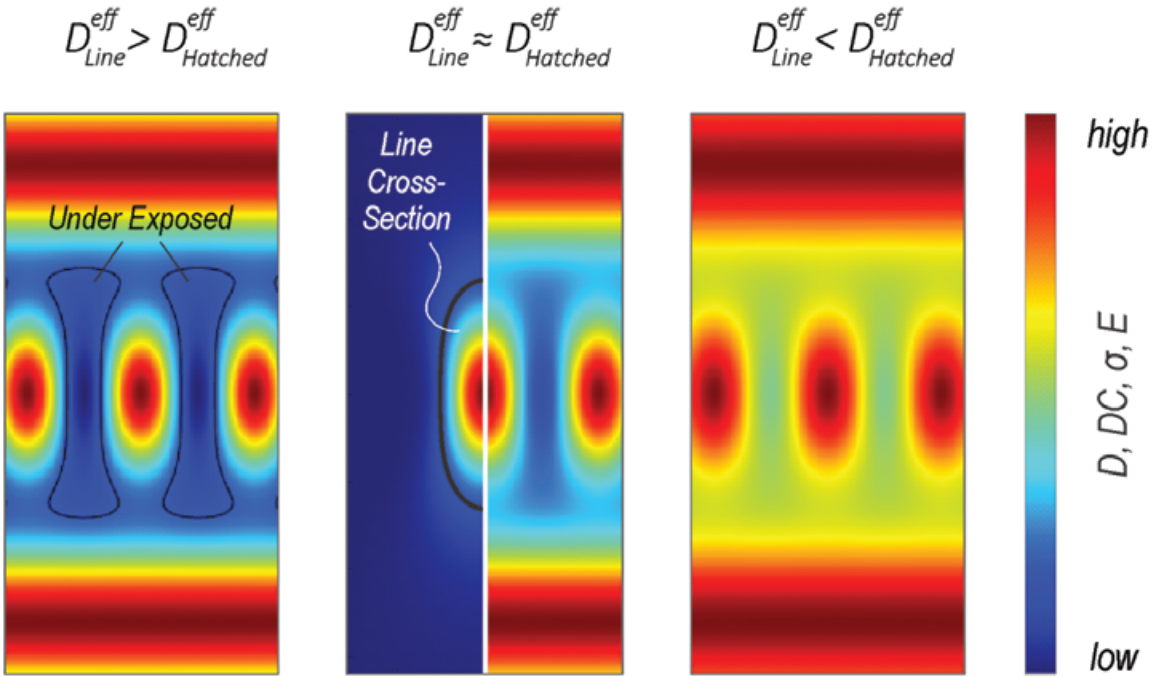
\includegraphics[height = 0.5\paperheight]{fig/2022-05-13_10-57-53.png}
                \end{minipage}
                \hfill
                \begin{minipage}[t]{0.45\linewidth}
                    \textbf{(б)} \\ 
                    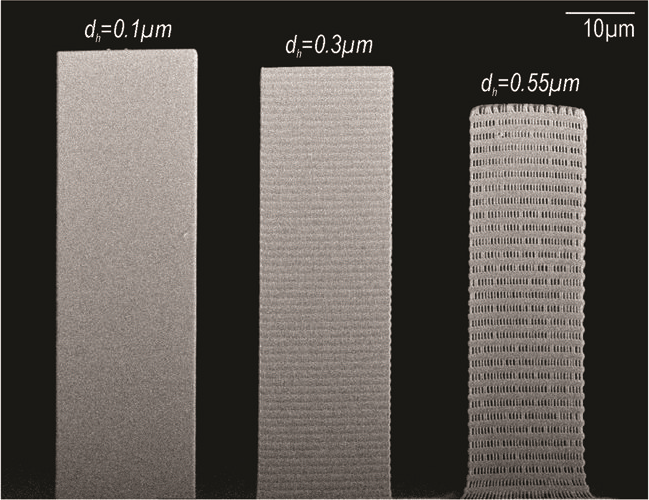
\includegraphics[height = 0.5\paperheight]{fig/d_h.png}
                \end{minipage}
                    \caption*{(a)Численный расчет размеров мульти-вокселей от расстояния $d_h$. (б)РЭМ снимок изготовленных 3D-микроструктур для механических испытаний\footcite{Mechrambald}.}
                    \label{fig:vox_dose_d_h}
            \end{figure}

\end{frame}

\begin{frame}{Алгоритм изготовления}
            \begin{figure}
                \begin{minipage}{0.4\linewidth}
                    \hspace*{-3em}\raisebox{0em}{
                    \begin{tikzpicture}
                        \node (a){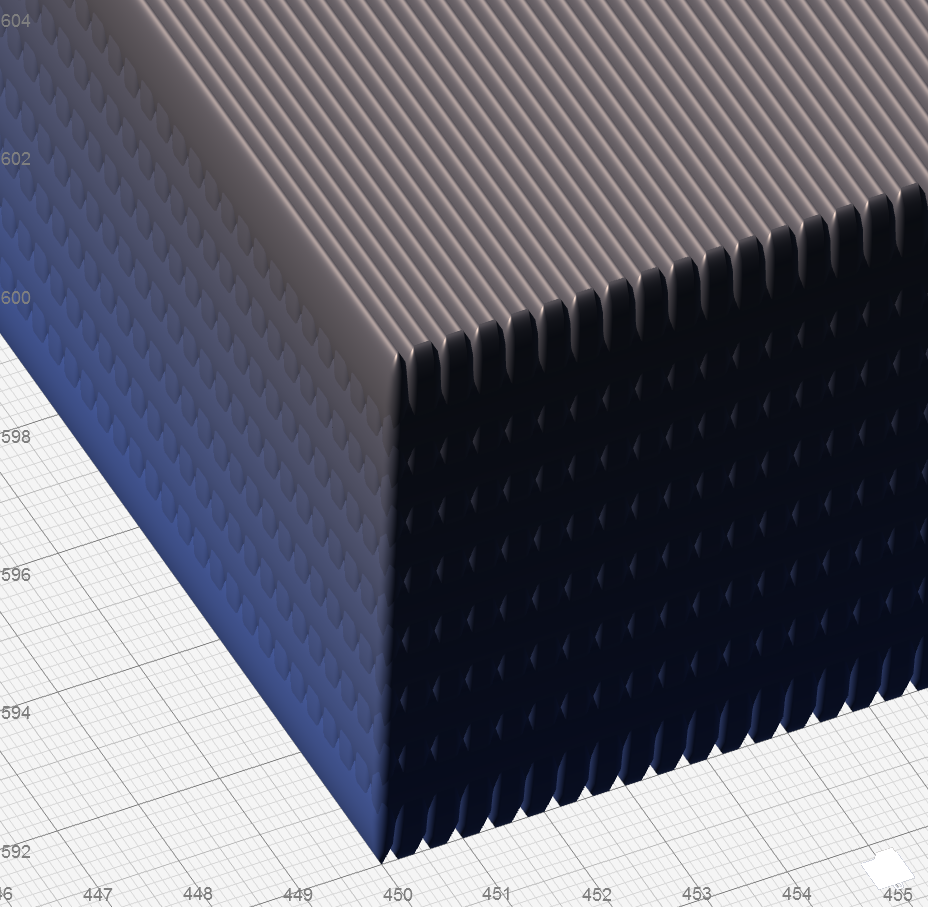
\includegraphics[trim=150 150 150 150, clip,height = 0.5\textheight]{fig/image10.png}};
                        \node at(a.north west)[xshift=0mm,yshift=0mm]{\textbf{(a)}};
                        \coordinate (len_h) at (-8mm,0);
                        \coordinate (len_v) at (0,8mm);
                        \coordinate (start_h) at (-5mm,2mm);
                        \coordinate (start_v) at (-1mm,10mm);
                        \draw[line,red,ultra thick] (start_h) -- +(len_h);
                        \draw[line,red,ultra thick] ($(start_h) + (0,-3mm)$) -- +(len_h);
                        \draw[line,red,ultra thick]  ($(start_h) + (len_h)$) -- +(0,-3mm) node[left,yshift=1mm] {$\boldsymbol{d_s = h(LP)}$} ;
                        \draw[<-, red,ultra thick] ($(start_h) + (len_h)+(0,-3mm)$) -- +(0,-5mm);
                        \draw[<-, red,ultra thick] ($(start_h) + (len_h)$) -- +(0,5mm);
                        
                        \draw[line,red,ultra thick] (start_v) -- +(len_v);
                        \draw[line,red,ultra thick] ($(start_v) + (3mm,0)$) -- +(len_v);
                        \draw[line,red,ultra thick]  ($(start_v) + (len_v)$) -- +(3mm,0) node[above,yshift=3mm] {$\boldsymbol{d_h = \, 200}$ \textbf{нм}} ;
                        \draw[<-, red,ultra thick] ($(start_v) + (len_v)+(3mm,0)$) -- +(5mm,0);
                        \draw[<-, red,ultra thick] ($(start_v) + (len_v)$) -- +(-5mm,0);
                    \end{tikzpicture}}
                \end{minipage}
                \begin{minipage}[с]{0.55\linewidth} 
                    \hspace*{-2em}\raisebox{-9em}{
                    \begin{tikzpicture}
                        \node (b) {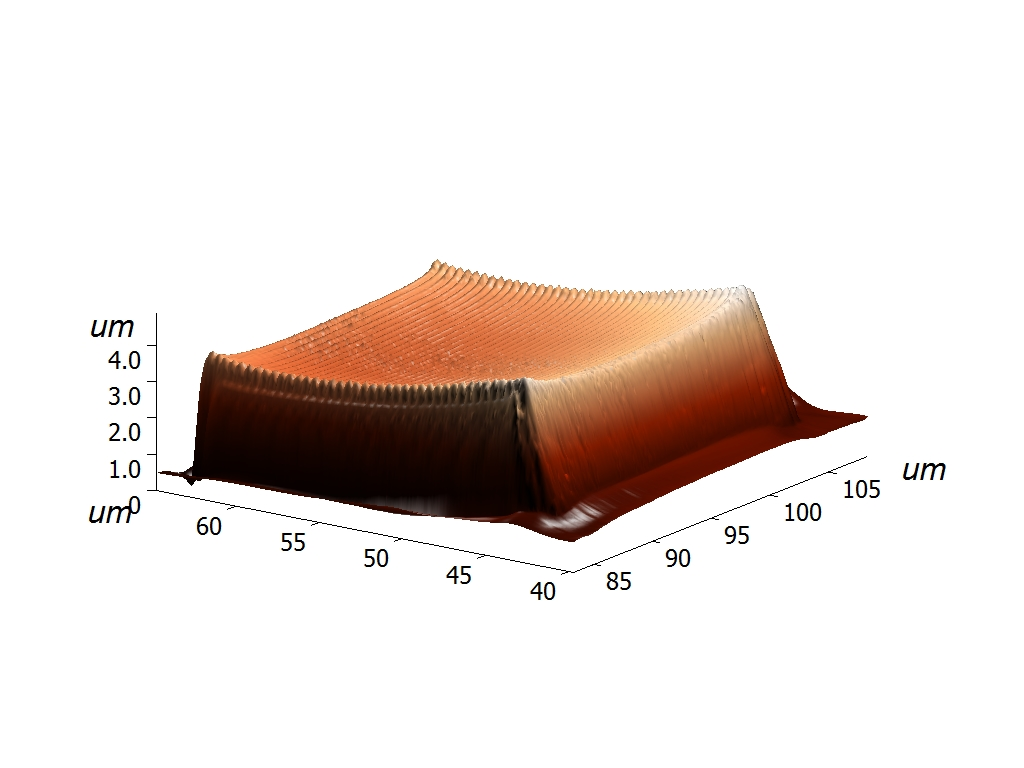
\includegraphics[trim=80 150 50 250, clip,width = 1.2\linewidth]{fig/3D_LP21_square_4.jpg}};
                        \node at(b.north west)[xshift=5mm,yshift=-5mm]{\textbf{(б)}};
                    \end{tikzpicture}}          
                \end{minipage}
                    \caption*{(а) 3D модель микроструктуры в программе DeScribe, визуализирующая алгоритм рисования.(б) 3D АСМ изображение 3D-микроструктуры высотой порядка 5 мкм}
                    \label{fig:vox_dose_d_h}
            \end{figure}

\end{frame}


\section{Исследование механических и оптических свойств}

\subsection{Наноиндентирование}

\begin{frame}{Наноиндентирование}
        \begin{figure}
            \begin{minipage}{0.45\linewidth}
                \begin{tikzpicture}
                    \node (a) {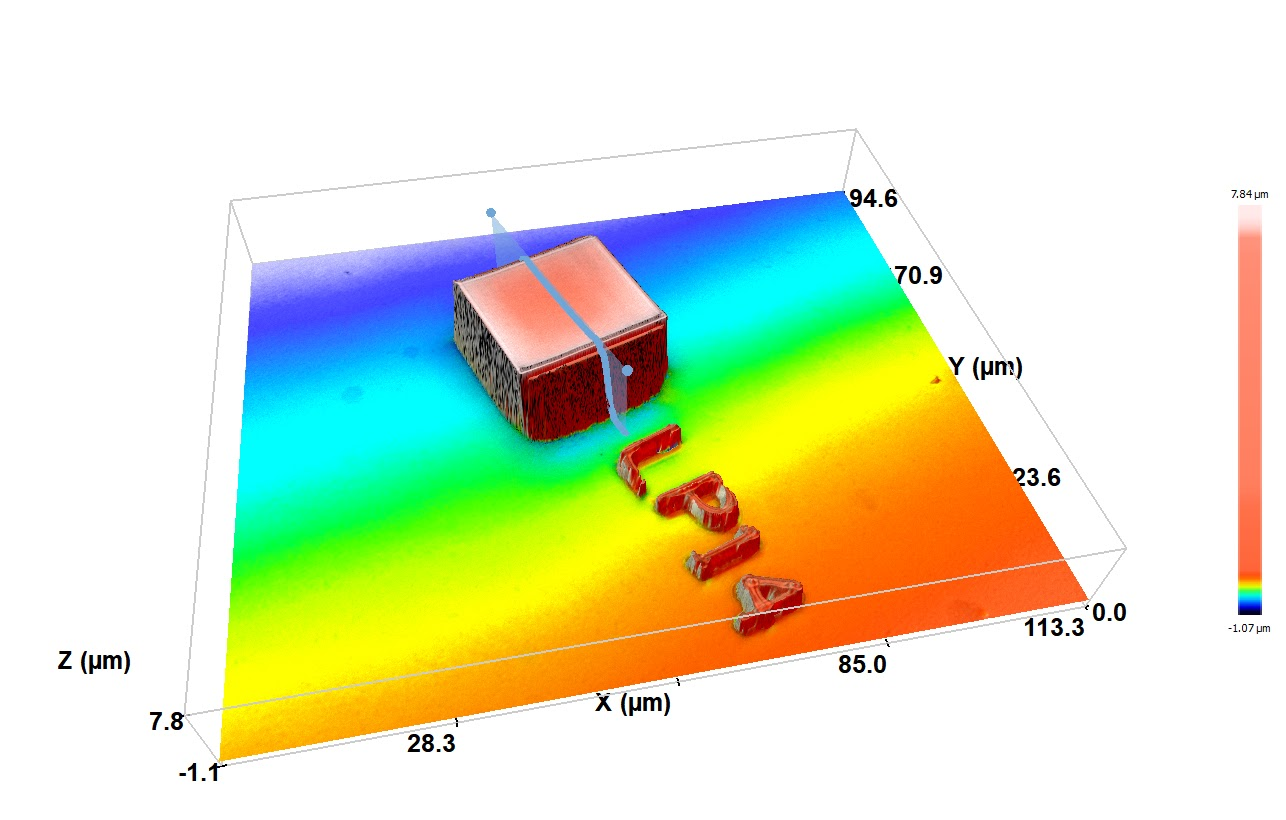
\includegraphics[trim=0 0 150 0,clip,width = 1\linewidth]{fig/image12.jpg}};
                    \node at (a.north west){\textbf{(a)}};
                    \node (square size) at (a.north)[yshift=-3mm] {$25 \times 25 \times 10$ мкм};
                \end{tikzpicture}
            \end{minipage}
            \hfill
            \begin{minipage}{0.45\linewidth}
                \begin{tikzpicture}%[node distance=0.24\linewidth and 0.24\linewidth]
                    \node (b){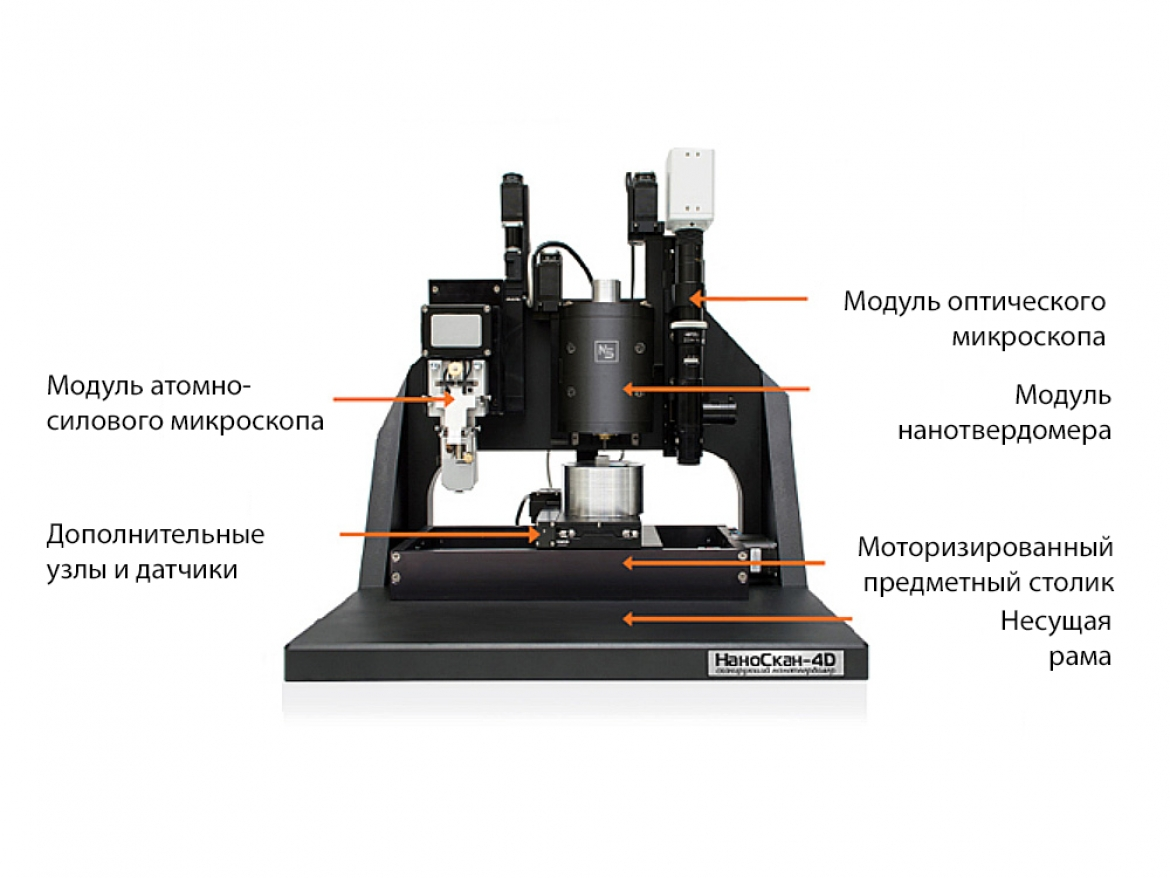
\includegraphics[trim=0 150 0 150, clip,width = 1\linewidth]{fig/image5.jpg}};
                    \node at (b.north west){\textbf{(б)}};
                \end{tikzpicture}
            \end{minipage}
                    % \coordinate (O) at (c.south east);
                    % % \fill [red] (A) ($(O) - (-25mm,10mm)$) circle (5pt);
                    % % \fill [red] (B) ($(O) - (-15mm,5mm)$) circle (5pt);
                    % % % \node[line,white] (scale) at (c.south east)[xshift=-15, yshift=15] {};
                    % % \draw[red,width=2mm] (scale) (A)--(B);
                    % % \node[white,above] (num_scale) at (scale.north) {$10$ мкм};
                \caption*{(a)~Снимок с оптического бесконтактного 3D профилометра Sensofar S Neox. Псевдоцветом визуализирована высота: от фиолетового (0 мкм) до красного (7,8 мкм).  (б)~Нанотвердомер <<Наноскан -- 4D>>}
            % \caption*{(a)~3D-микроструктура. (б)~Алмазный плоский штамп. (с)~ нагрузочная/разгрузочная кривая.}
        \end{figure}
\end{frame}



\begin{frame}{Наноиндентирование}
        \begin{figure}
                \begin{tikzpicture}%[node distance=0.24\linewidth and 0.24\linewidth]
                    \node (b) [below= of a,yshift=10mm]{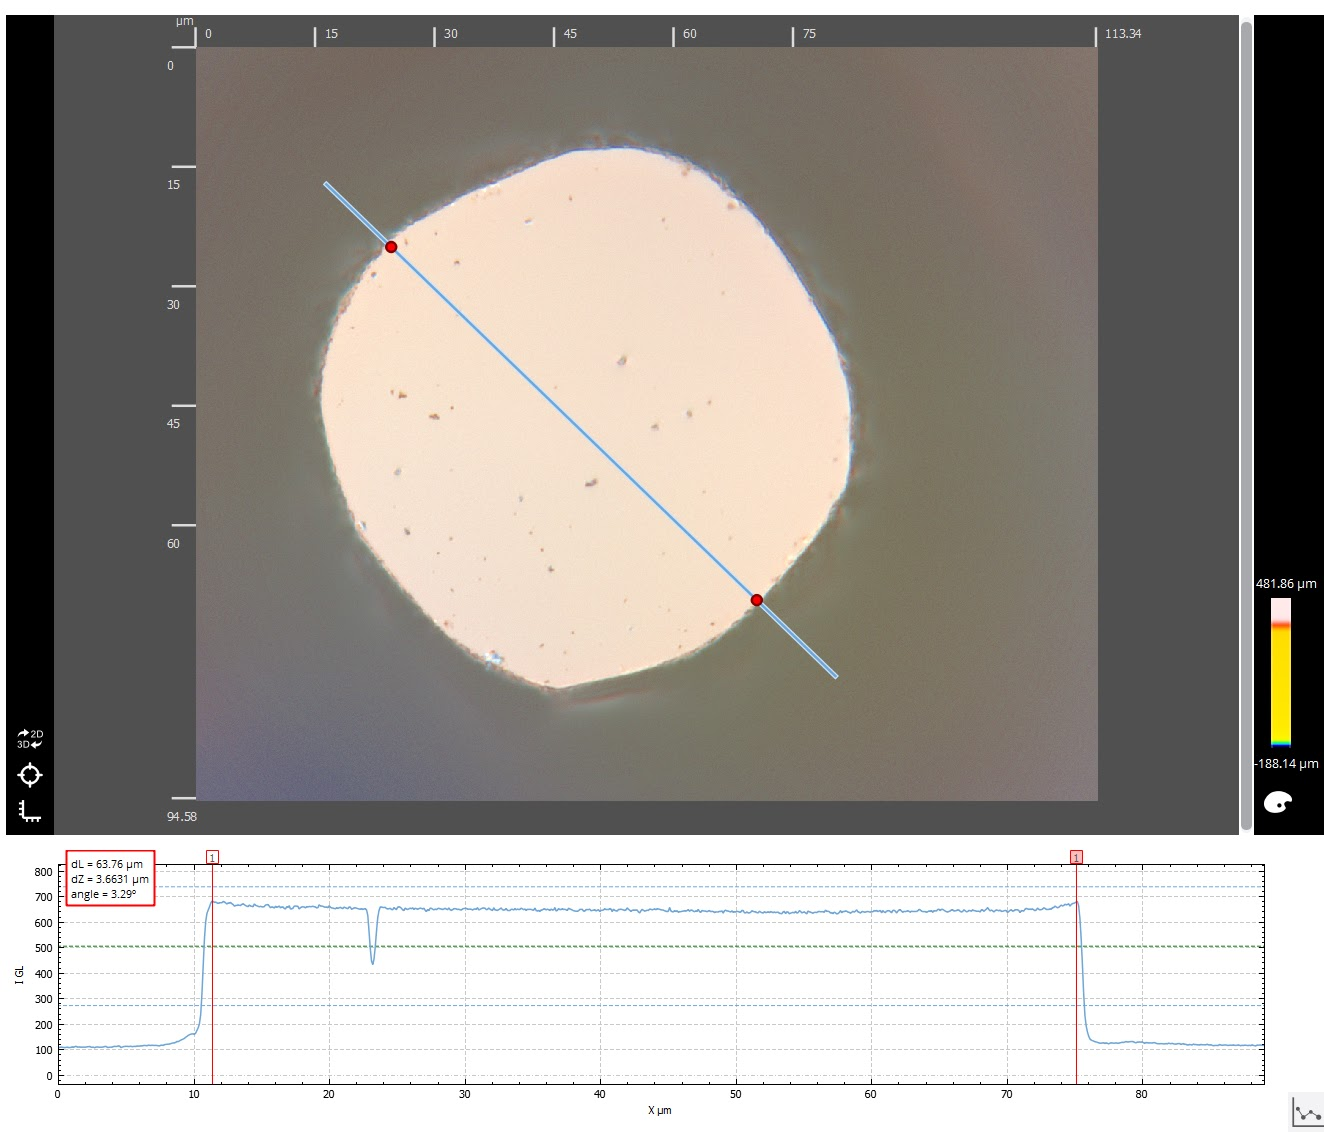
\includegraphics[trim=150 350 250 100,clip,width = 0.5\linewidth]{fig/image11.jpg}};
                    \node (indent size) at (b.center) {$\sim \, 70$ мкм};
                \end{tikzpicture}
                \caption*{Плоский алмазный штамп.}
            % \caption*{(a)~3D-микроструктура. (б)~Алмазный плоский штамп. (с)~ нагрузочная/разгрузочная кривая.}
        \end{figure}
\end{frame}

\begin{frame}{Наноиндентирование}
    \begin{columns}
        \column{0.35\linewidth}
        {Параметры испытаний:
        \begin{itemize}
            \item Глубина вдавливания 800~нм
            \item Время нагружения/разгружения 100~с
            \item Время выстаивания 10~с
        \end{itemize}
        }
        \column{0.65\linewidth}
        {
        \begin{figure}%\hspace*{0em}\raisebox{15em}{
                \begin{tikzpicture}
                    \node (c) [right= of a,xshift=-10mm] {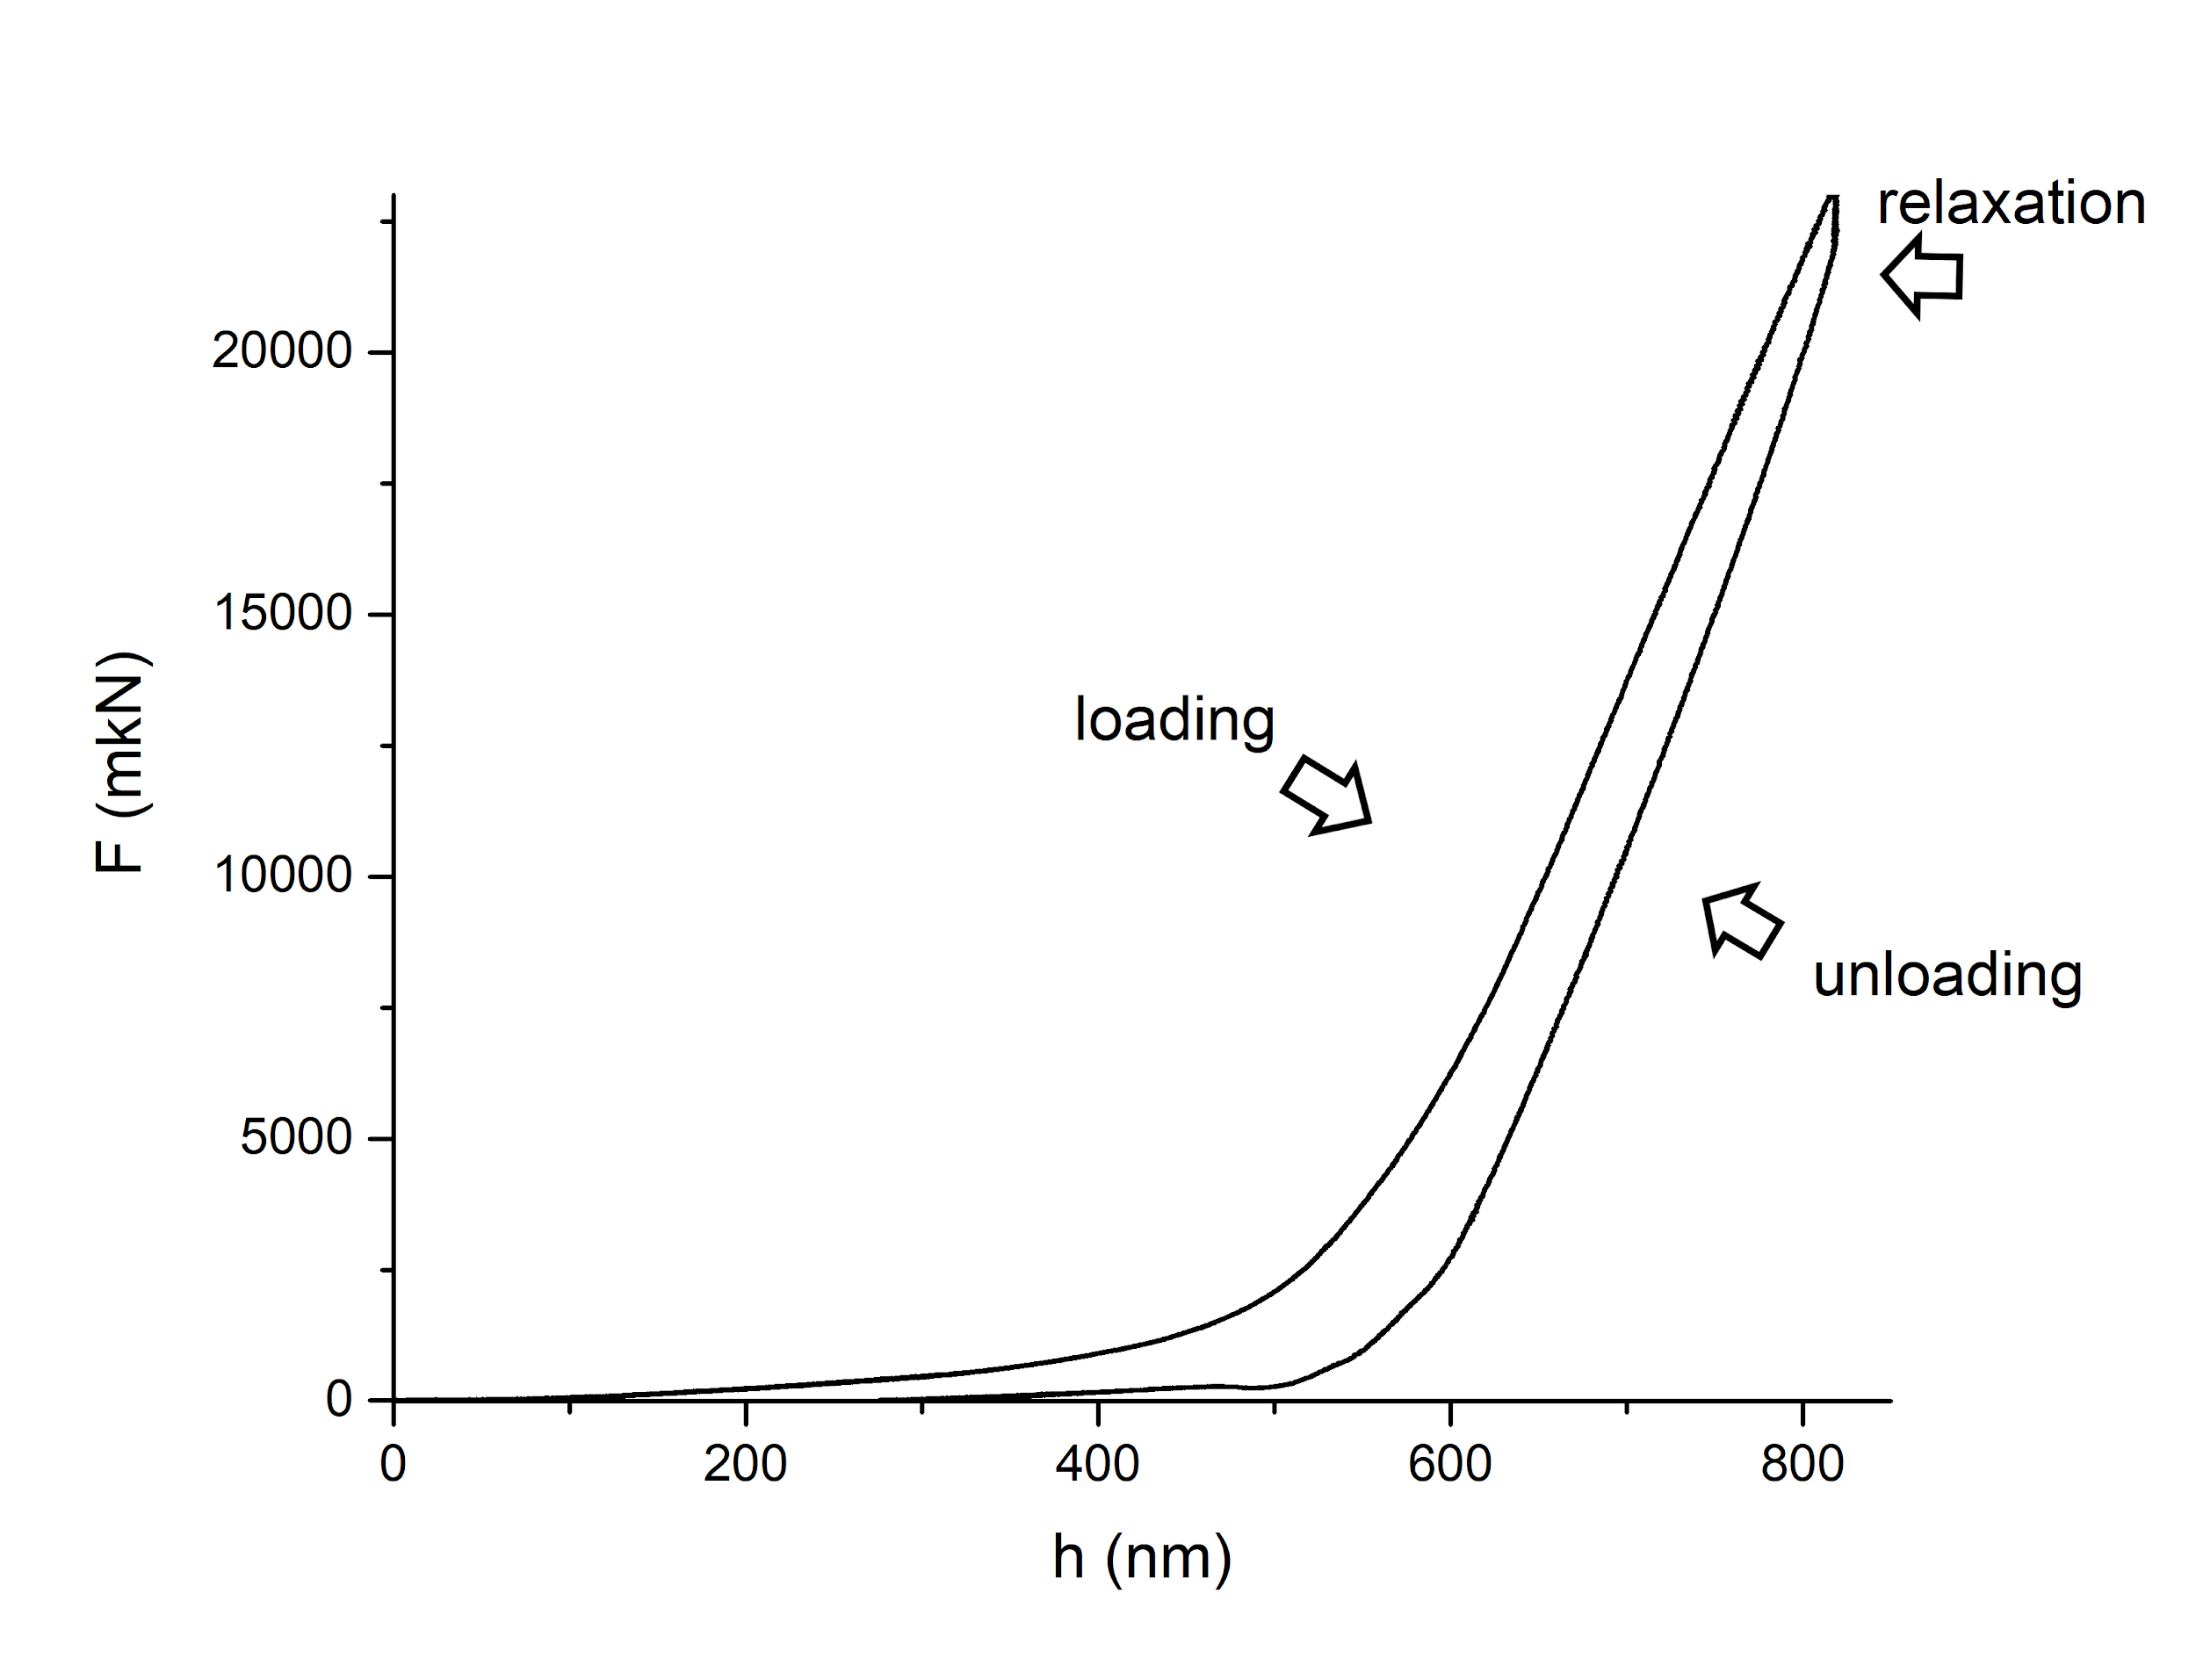
\includegraphics[trim=100 100 50 200, clip,width = 0.8\linewidth]{fig/image21.png}};
                    \node (square) at (c.north west)[xshift=75, yshift=-20] {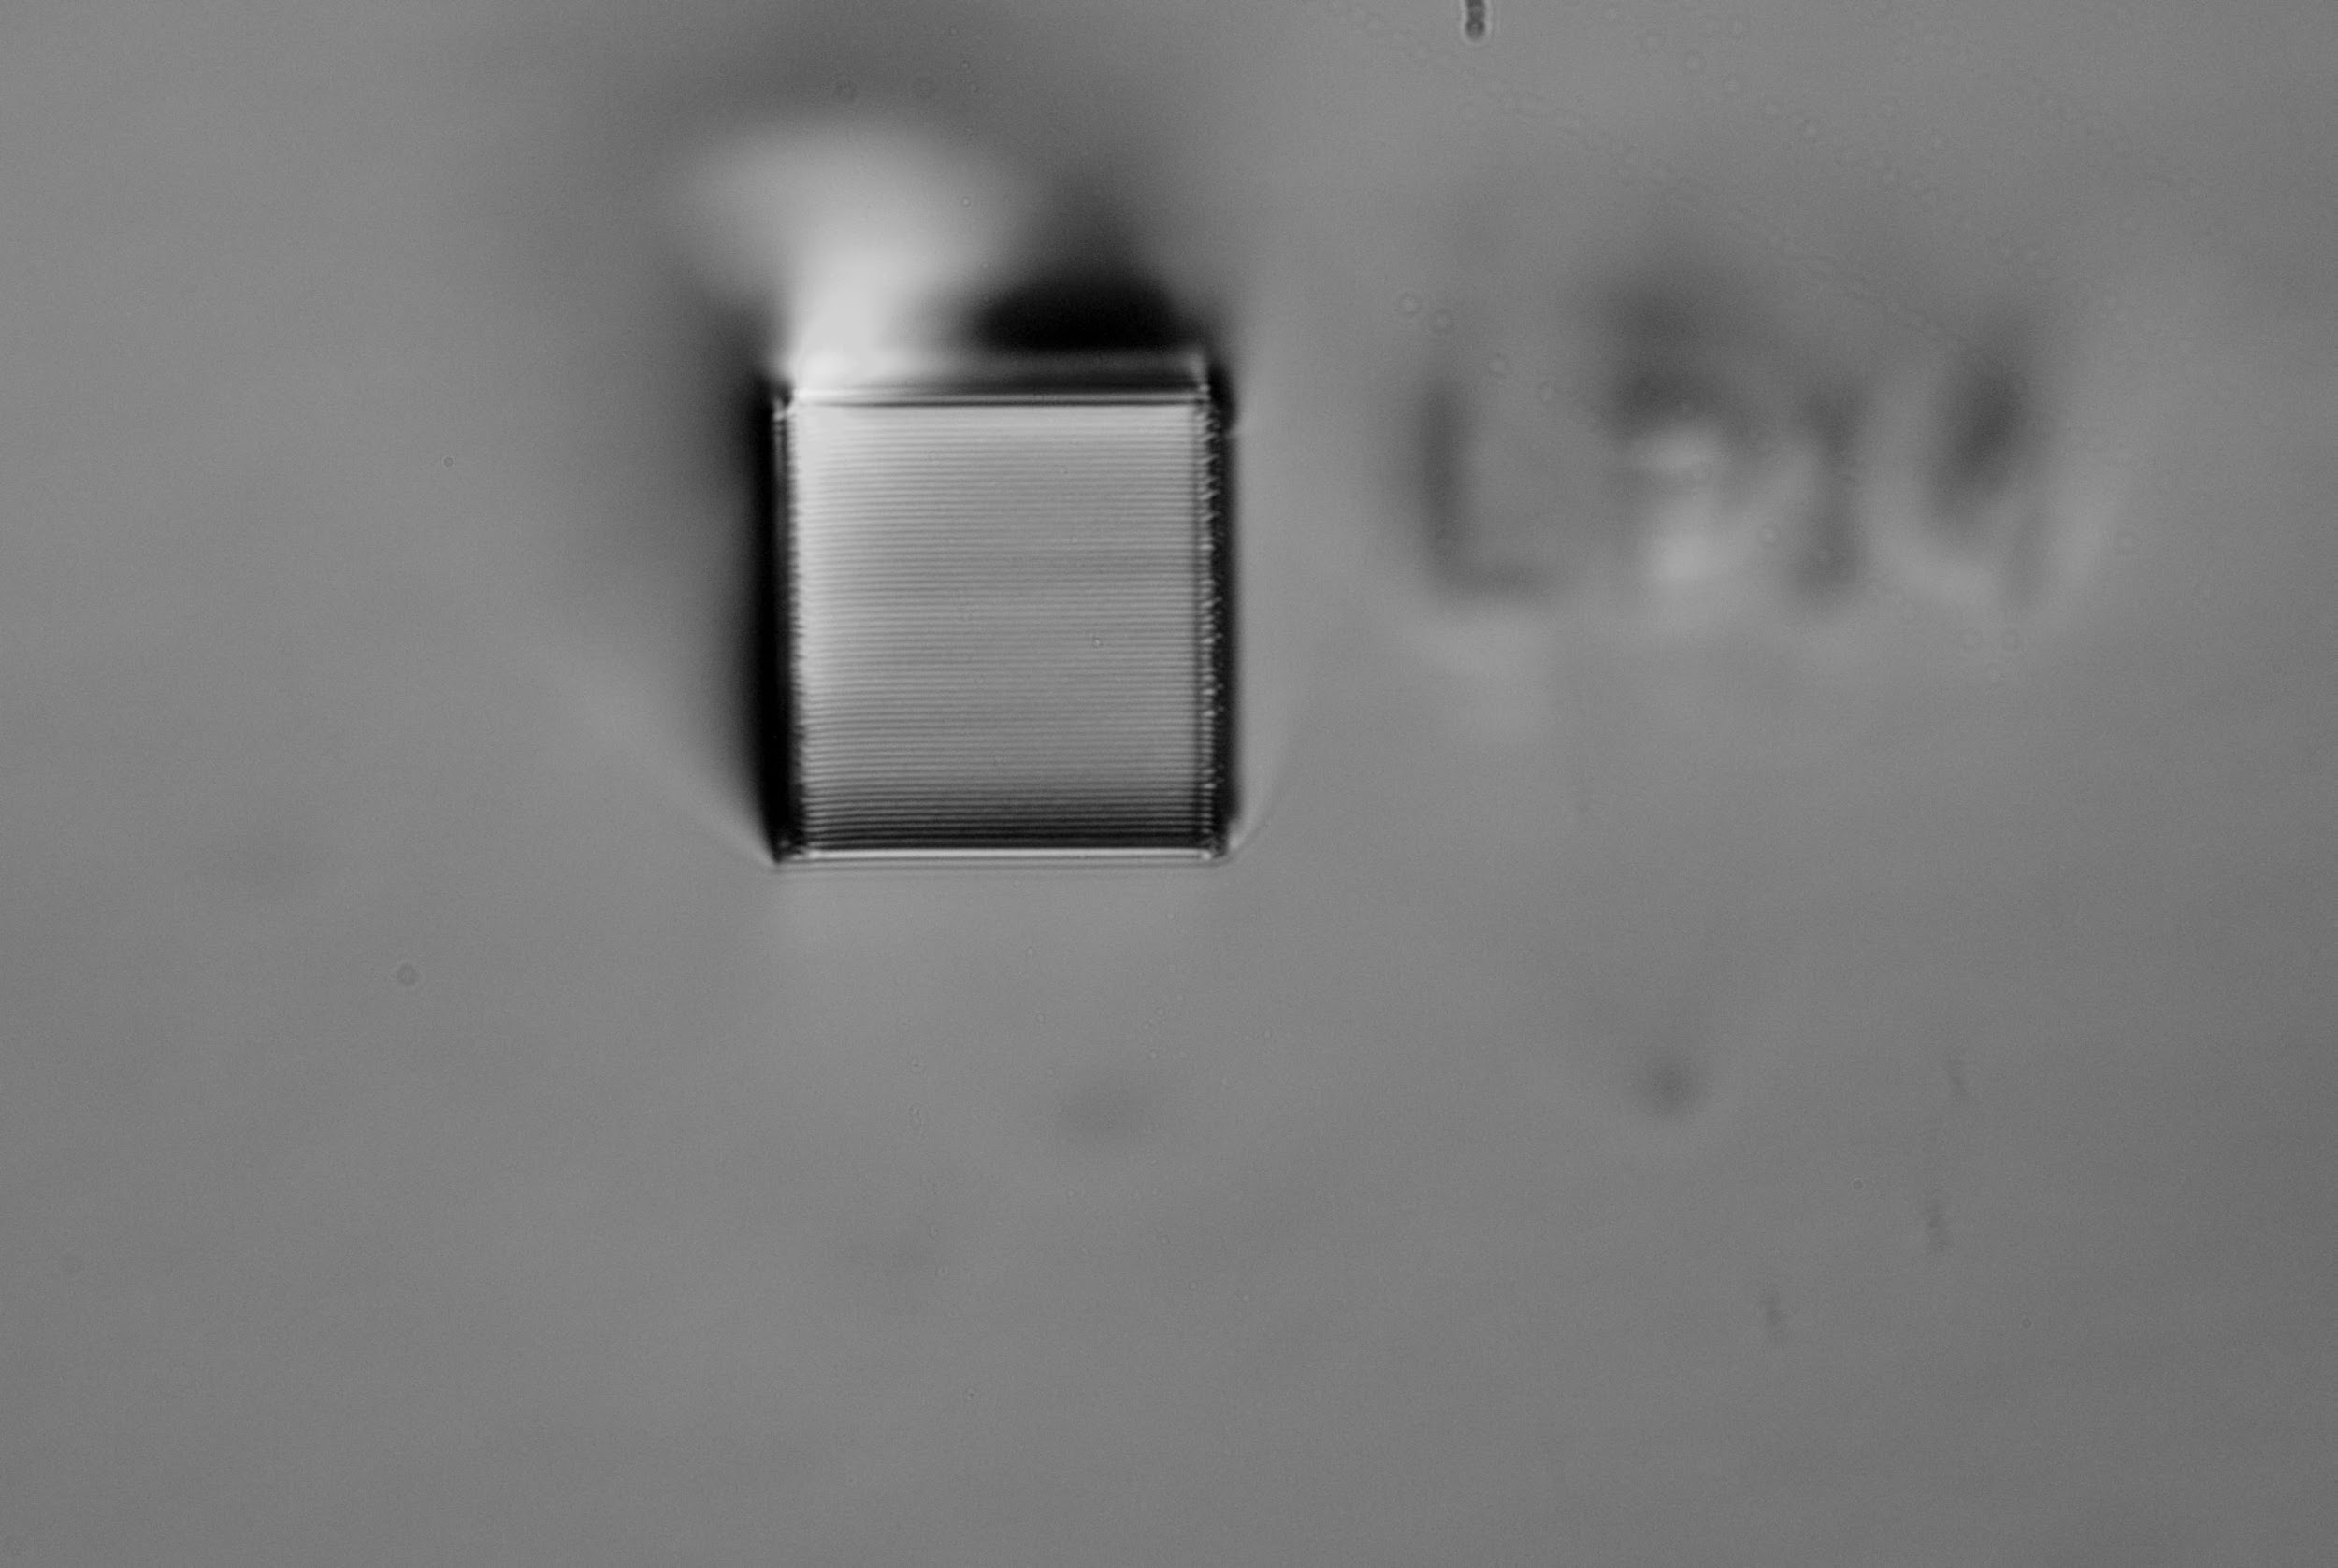
\includegraphics[trim=550 550 0 0, clip,width = 0.25\linewidth]{fig/image14.jpg}};
                    \draw[thick,red] (square.center)[xshift=-5mm,yshift=-1.0mm] circle [radius=8.4mm] node [above,align=center,yshift=10mm] {размер штампа};
                    \node[draw] at (c.east)[xshift=10mm,yshift=0mm]{$E_r= \frac{dF}{dh}\frac{t}{A}$};
                    % \node at (c.north east)[xshift=5mm,yshift=5mm]{$E_r= \frac{dF}{dh}\frac{t}{A}$};
                \end{tikzpicture}
                    % \coordinate (O) at (c.south east);
                    % % \fill [red] (A) ($(O) - (-25mm,10mm)$) circle (5pt);
                    % % \fill [red] (B) ($(O) - (-15mm,5mm)$) circle (5pt);
                    % % % \node[line,white] (scale) at (c.south east)[xshift=-15, yshift=15] {};
                    % % \draw[red,width=2mm] (scale) (A)--(B);
                    % % \node[white,above] (num_scale) at (scale.north) {$10$ мкм};
            \caption*{Силовая нагрузочная /разгрузочная кривая.}
            % \caption*{(a)~3D-микроструктура. (б)~Алмазный плоский штамп. (с)~ нагрузочная/разгрузочная кривая.}
        \end{figure}
        }
    \end{columns}
\end{frame}


\subsection{Рамановская спектроскопия}

\begin{frame}{Рамановская спектроскопия}
        \begin{figure}
            \begin{minipage}{0.45\linewidth}
                \begin{tikzpicture}
                    \node  (a) {
\includegraphics[height =0.48\textheight]{fig/image4.png}};
                    \node at (a.north west) {(a)};
                \end{tikzpicture}
            \end{minipage}
            \hfill
            \begin{minipage}{0.45\linewidth}
                \begin{tikzpicture}
                    \node (b) {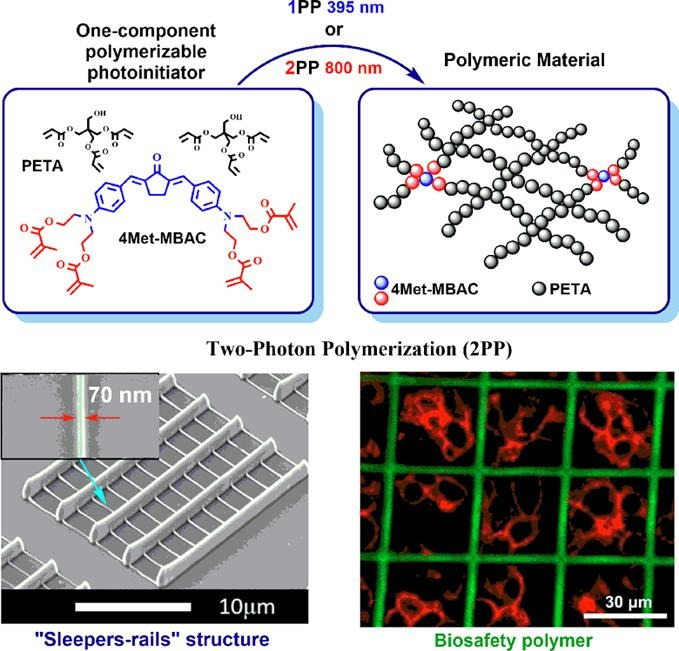
\includegraphics[trim=85 80 0 21,clip,height =0.48\textheight]{fig/1-s2.0-S0014305721006510-ga1_lrg.jpg}};
                    \node at (b.north west) {(б)};
                \end{tikzpicture}
            \end{minipage}
            % \hfill
            % \begin{minipage}{0.45\linewidth}
            %     \caption*{(a) Формулы используемого фотоинициатора(4MetBAC) и мономера(PETA)\footcite{4metbac} (б) спектр поглощения 4MetBAC и MBAC\footcite{4metbac} (с) Рамановский спектр{4metbac}}
            % \end{minipage}            
            \caption*{(a)~Формулы используемых веществ: фотоинициатора (4Met-BAC) и мономера (PETA). (б)~Полимерная цепочка. Цветом обозначены следующие вещества: MBAC~(cиний), (мет)акрилатные группы~(красный), PETA~(серый)\footcite{4metbac}.}
        \end{figure}
\end{frame}

\begin{frame}{Рамановская спектроскопия}
        \begin{figure}
                \begin{tikzpicture}
                    \node (b) {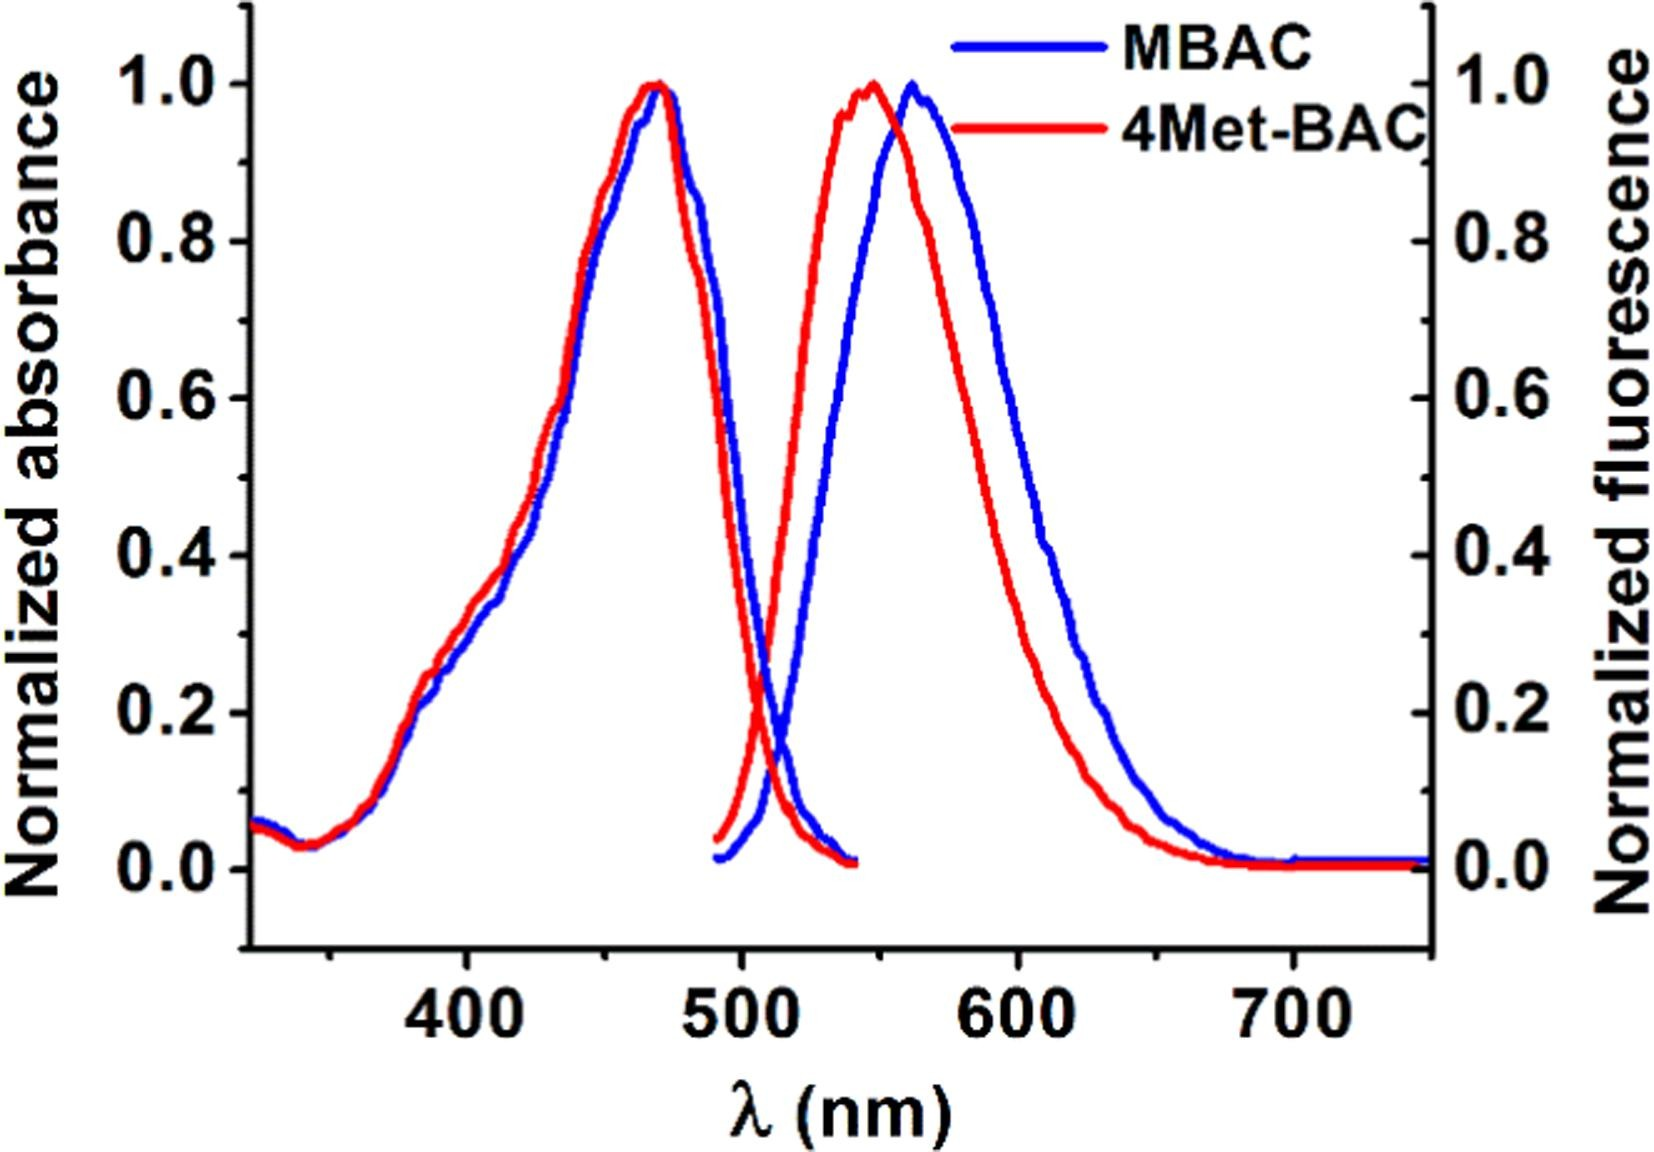
\includegraphics[width =0.5\linewidth]{fig/1-s2.0-S0014305721006510-gr3_lrg (1).jpg}};
                    \draw[<-,red,ultra thick] (11.5mm,-5mm) -- +(0,15mm);
                \end{tikzpicture}
            \caption*{Спектры поглощения и флюоресценции 4Met-BAC и MBAC\footcite{4metbac}}
        \end{figure}
\end{frame}

\begin{frame}{Рамановская спектроскопия}
        \begin{columns}
        \column{0.35\linewidth}
        {Параметры снятия спектра:
        \begin{itemize}
            \item Длина волны лазера 633~нм
            \item Мощность лазера 3,5~мВт
            \item Время экспозиции 70~с
        \end{itemize}
        }
        \column{0.65\linewidth}
        {
        \begin{figure}
                \begin{tikzpicture}
                    \node (c) {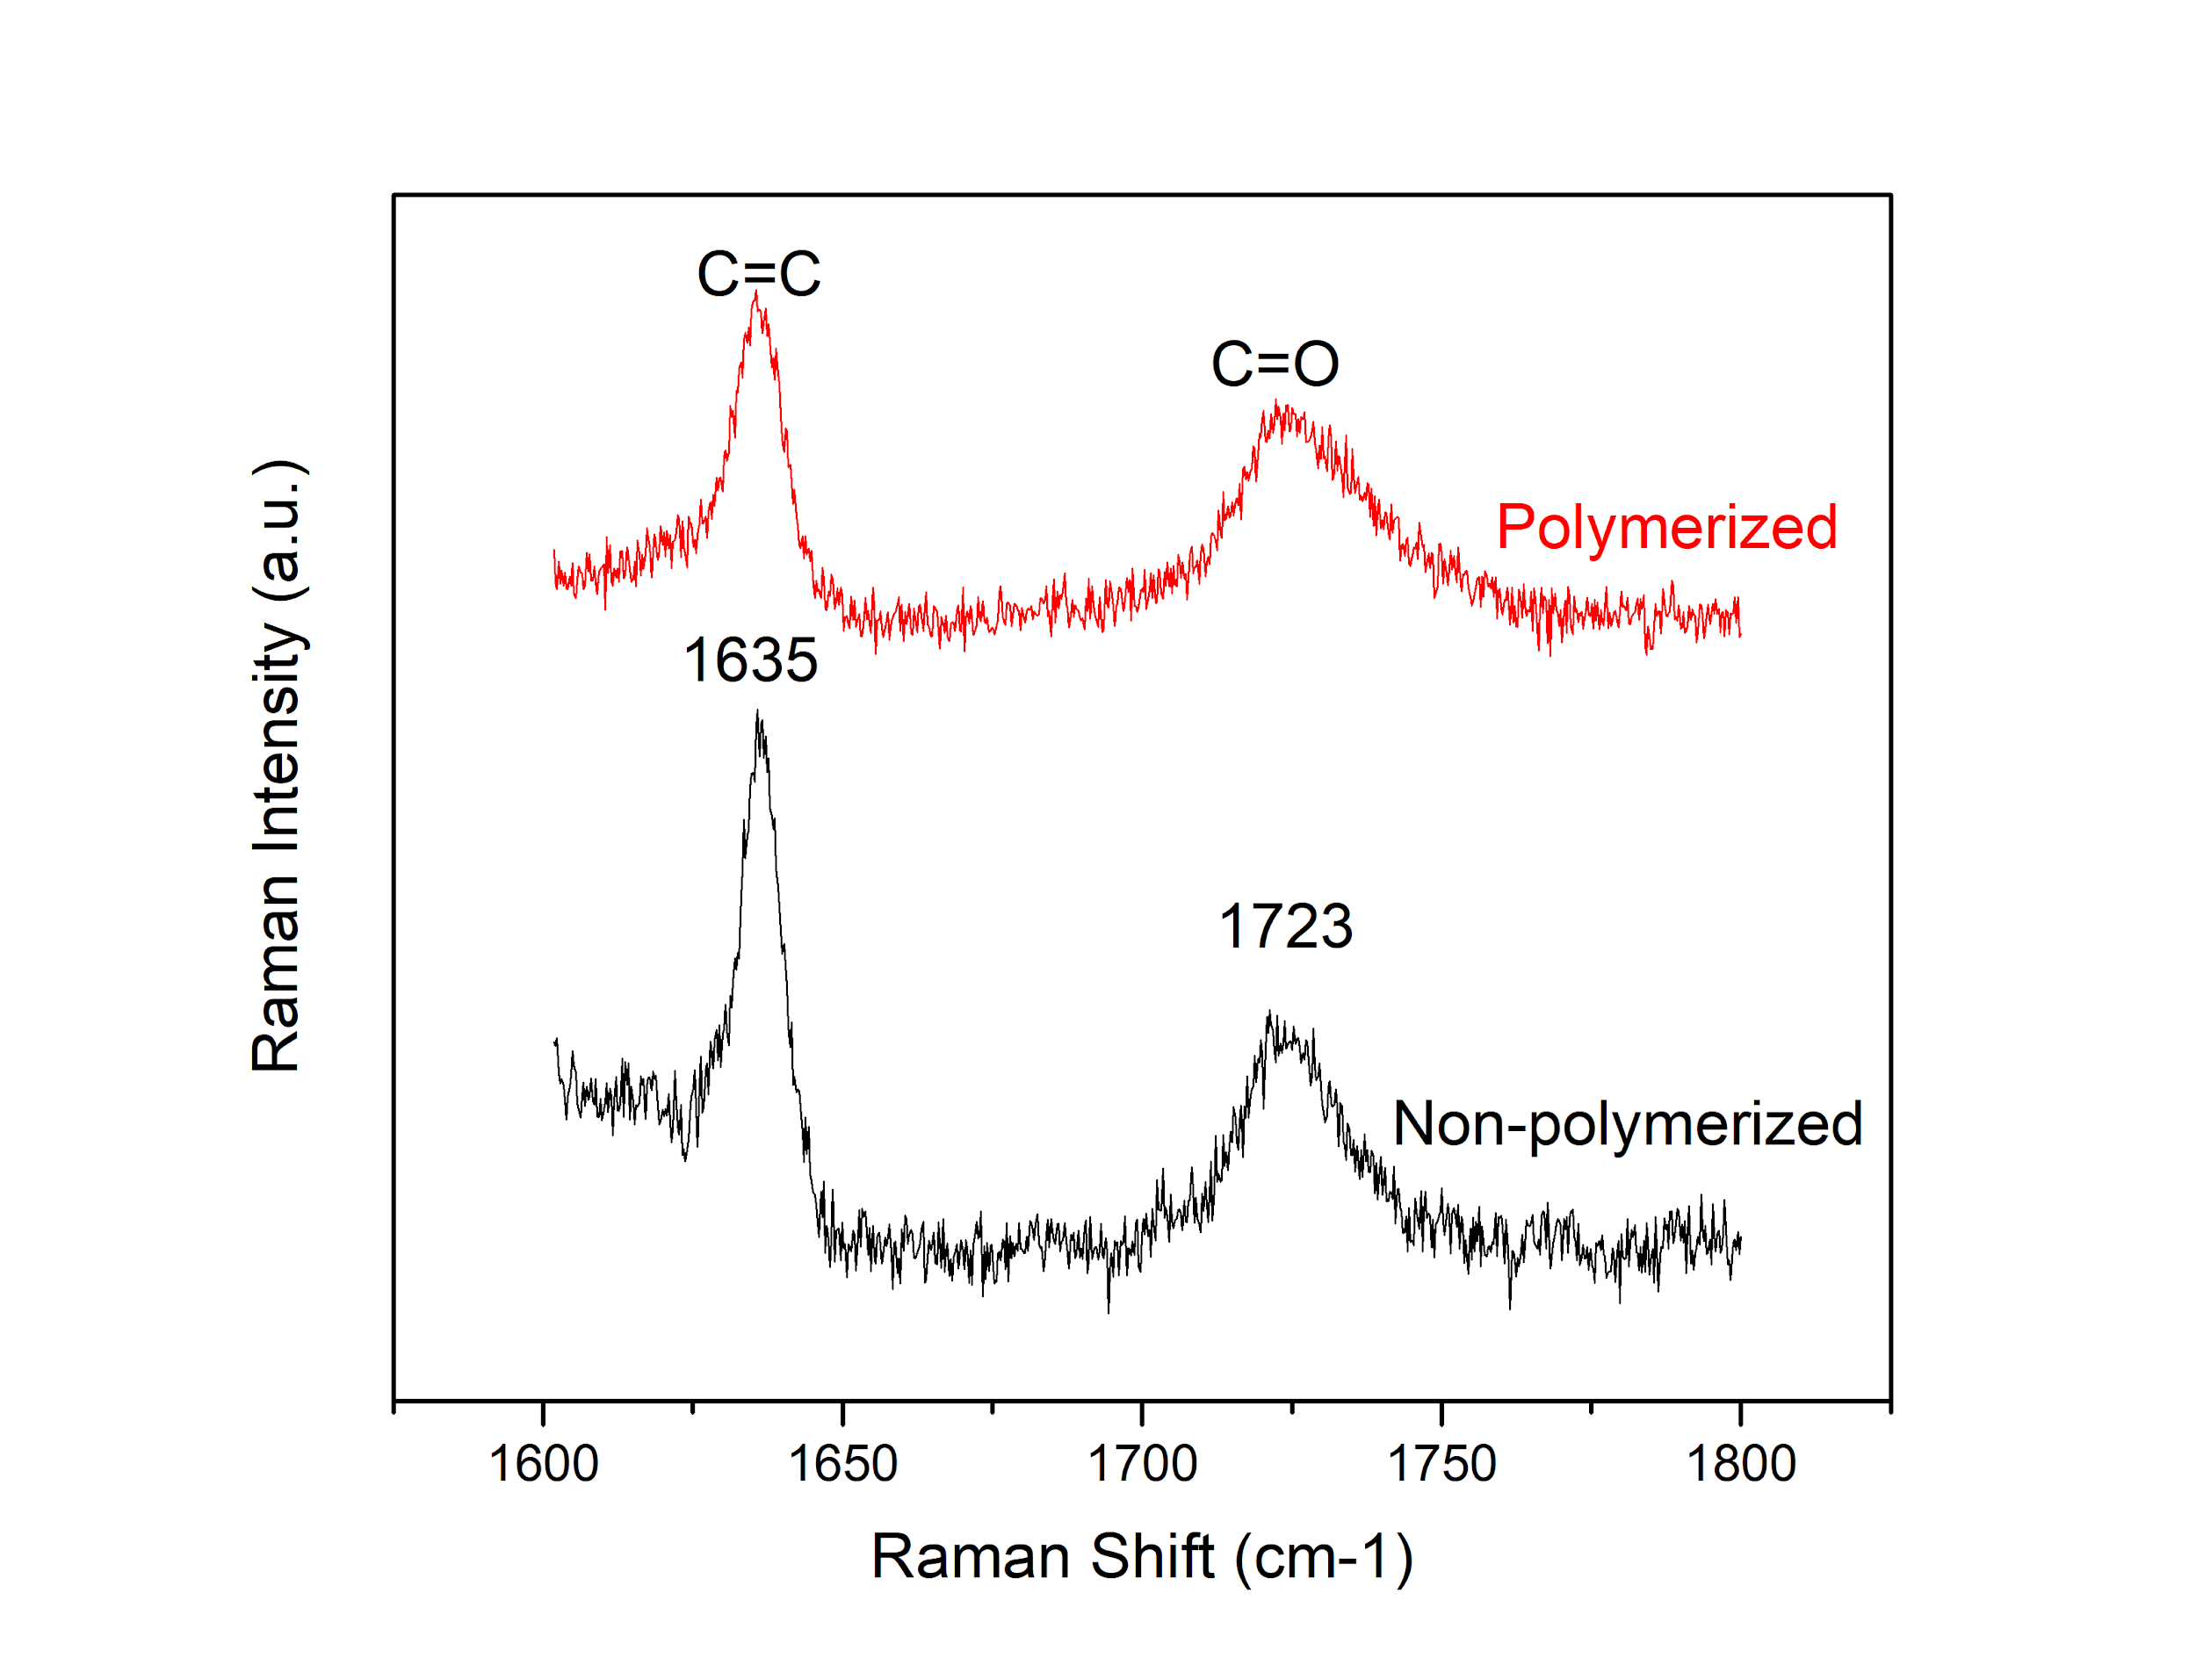
\includegraphics[trim=250 100 150 150, clip,width =0.6\linewidth]{fig/image19.png}};
                    \node (square)  at (c.north east)[xshift=-8mm,yshift=-4mm] {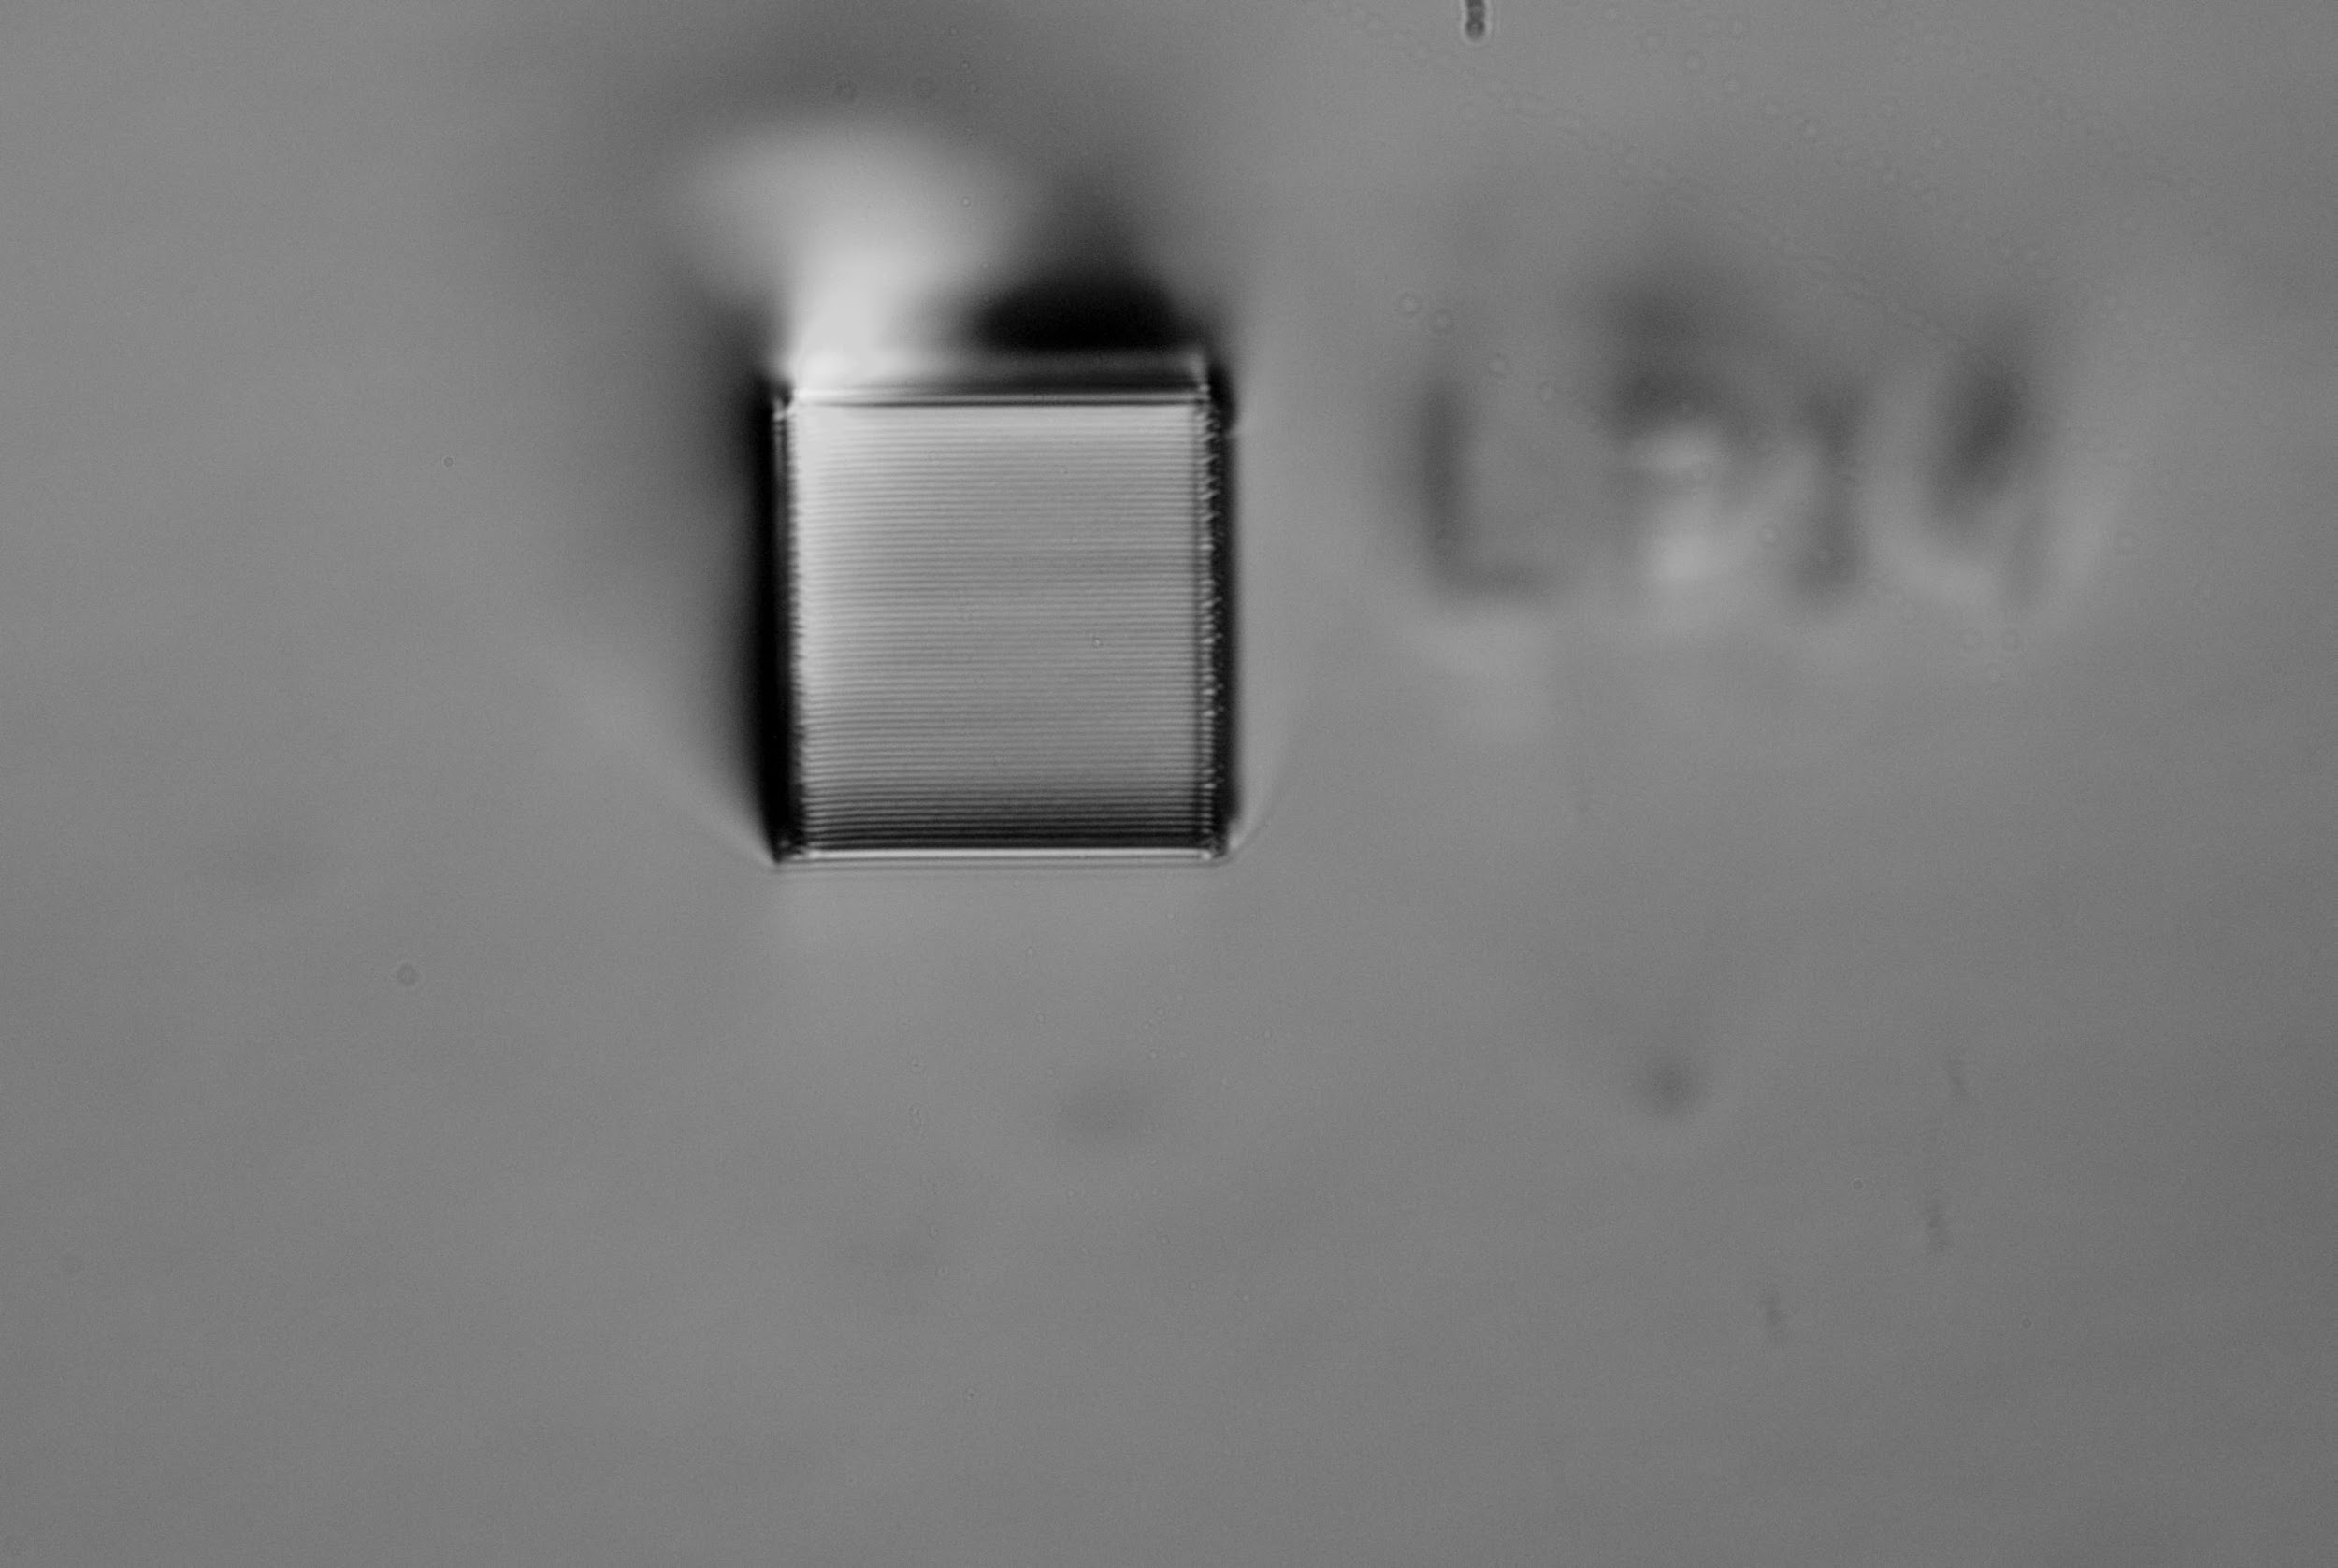
\includegraphics[trim=550 550 0 0, clip,width = 0.2\linewidth]{fig/image14.jpg}};
                    \draw[red,fill] (square.center)[xshift=-4.2mm,yshift=-0.9mm] circle [radius = 0.47mm] node [above,align=center,yshift=9mm] {размер фокального} node [above,align=center,yshift=5mm]{лазерного пятна};
                    \draw[<-,red,thick] (16.5mm,18.5mm) -- +(0,5mm);
                \end{tikzpicture}
                % \caption*{(a) Формулы используемого фотоинициатора(4MetBAC) и мономера(PETA) (б) спектр поглощения 4MetBAC и MBAC  (с) Рамановский спектр}
            % \hfill
            % \begin{minipage}{0.45\linewidth}
            %     \caption*{(a) Формулы используемого фотоинициатора(4MetBAC) и мономера(PETA)\footcite{4metbac} (б) спектр поглощения 4MetBAC и MBAC\footcite{4metbac} (с) Рамановский спектр{4metbac}}
            % \end{minipage}            
            \caption*{Рамановский спектр неполимеризованной фотокомпозциии и 3D-микроструктуры}
        \end{figure}
        }
    \end{columns}
\end{frame}
% \begin{frame}
% \frametitle{Blocks of Highlighted Text}
% \begin{block}{Regular Block}
% Lorem ipsum dolor sit amet, consectetur adipiscing elit. Integer lectus nisl, ultricies in feugiat rutrum, porttitor sit amet augue. Aliquam ut tortor mauris. Sed volutpat ante purus, quis accumsan dolor.
% \end{block}

% \begin{exampleblock}{Example Block}
% Pellentesque sed tellus purus. Class aptent taciti sociosqu ad litora torquent per conubia nostra, per inceptos himenaeos. Vestibulum quis magna at risus dictum tempor eu vitae velit.
% \end{exampleblock}

% \begin{alertblock}{Alert Block}
% Suspendisse tincidunt sagittis gravida. Curabitur condimentum, enim sed venenatis rutrum, ipsum neque consectetur orci, sed blandit justo nisi ac lacus.
% \end{alertblock}
% \end{frame}


% \begin{frame}
% \frametitle{Colors}

% You can use main official predefined colors 
% \textcolor{ITMOblue}{ITMOblue} and \textcolor{ITMOred}{ITMOred}, and also
%  \textcolor{ITMOorange}{ITMOorange}, \textcolor{ITMOsky}{ITMOsky}, \textcolor{ITMOpistachio}{ITMOpistachio}, \textcolor{ITMOaqua}{ITMOaqua}, \textcolor{ITMOice}{ITMOice}, \textcolor{ITMOgold}{ITMOgold}, \textcolor{ITMOyellow}{ITMOyellow}, \textcolor{ITMOtomato}{ITMOtomato}, \textcolor{ITMOgreen}{ITMOgreen}.

% \end{frame}



% \subsection{Using columns}


% \begin{frame}
% \frametitle{Multiple Columns}
% \begin{columns}[c] 

% \column{.45\textwidth}{
%     \begin{enumerate}
%         \item First item
%         \item Second item
%         \item Third item
%     \end{enumerate}
% }

% \column{.45\textwidth}{
%     \begin{itemize}
%         \item Some item
%         \item Another item
%         \item Also item
%     \end{itemize}
% }

% \end{columns}
% \end{frame}


% \subsection{Tables}


% \begin{frame}
% \frametitle{Table}

% % Лучше не использовать table в презентациях, только tabular. А описание таблиц делать руками.

% \begin{table} 
% \caption*{Multiplication table of complex numbers}
% \begin{tabular}{r | r r r r r} 
% $a \times b$ & $0$ &  $1$ &  $i$ & $-1$ & $-i$ \\ \hline
%          $0$ & $0$ &  $0$ &  $0$ &  $0$ &  $0$ \\
%          $1$ & $0$ &  $1$ &  $i$ & $-1$ & $-i$ \\
%          $i$ & $0$ &  $i$ & $-1$ & $-i$ &  $1$ \\
%         $-1$ & $0$ & $-1$ & $-i$ &  $1$ &  $i$ \\
%         $-i$ & $0$ & $-i$ &  $1$ &  $i$ & $-1$ \\
% \end{tabular}
% \end{table}
% \end{frame}


% \subsection{Theorems and Equations}


% \begin{frame}
% \frametitle{Theorem}
% \begin{theorem}[Fermat's Last Theorem]
% \begin{equation}
%     \forall n, x, y, z \in \mathbb{N}: \mathbf{n > 2} \Rightarrow x^n + y^n \neq z^n
% \end{equation}
% \end{theorem}
% I have discovered a truly remarkable proof of this theorem which this frame is too small to contain.
% \end{frame}


% \subsection{Figures}


% \begin{frame}
% \frametitle{Figure example}
% \begin{figure}
%     \includegraphics[scale=.3]{fig/parabola.png}
%     \caption*{Parabola with focus and directrix}
% \end{figure}
% \end{frame}


\section{Заключение}

\begin{frame}{Результаты}

        \begin{figure}
            \begin{tikzpicture}%[node distance=0.22 \linewidth and 0.22 \linewidth]
                \node (a)% at (0,30mm)
                {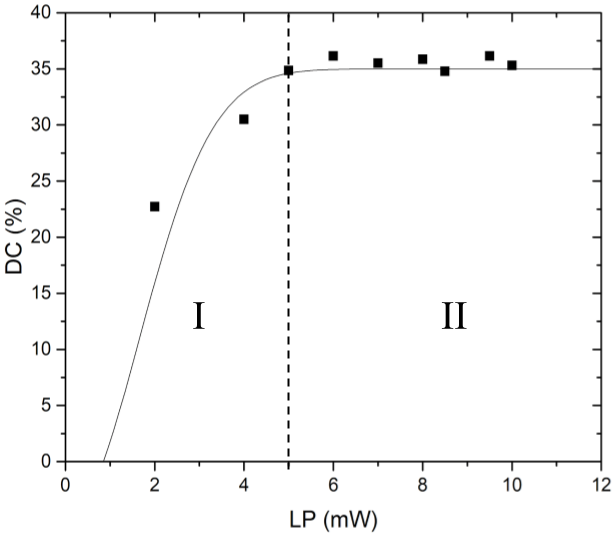
\includegraphics[ height= 0.6 \textheight]{fig/DC(LP).png}};
                \node (b) [right= of a][xshift = 0mm] {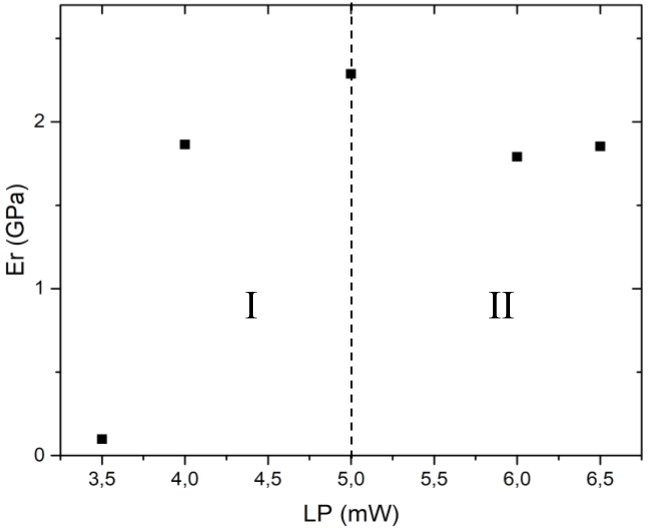
\includegraphics[height = 0.6 \textheight]{fig/Er(LP).png}};
                \node at (a.north west){(a)};
                \node at (b.north west){(б)};
                \node (bri) at (a.south east)[xshift=7mm,yshift=10mm]{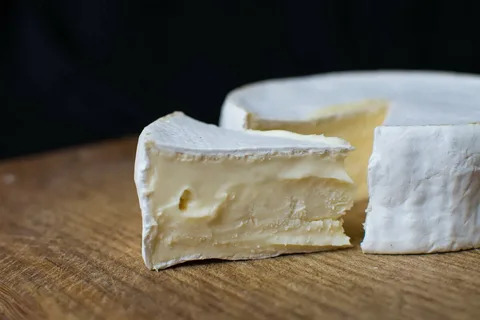
\includegraphics[width=10mm]{fig/bri.jpg}};
                \node (parm) at (a.north east)[xshift=7mm,yshift=-7mm]{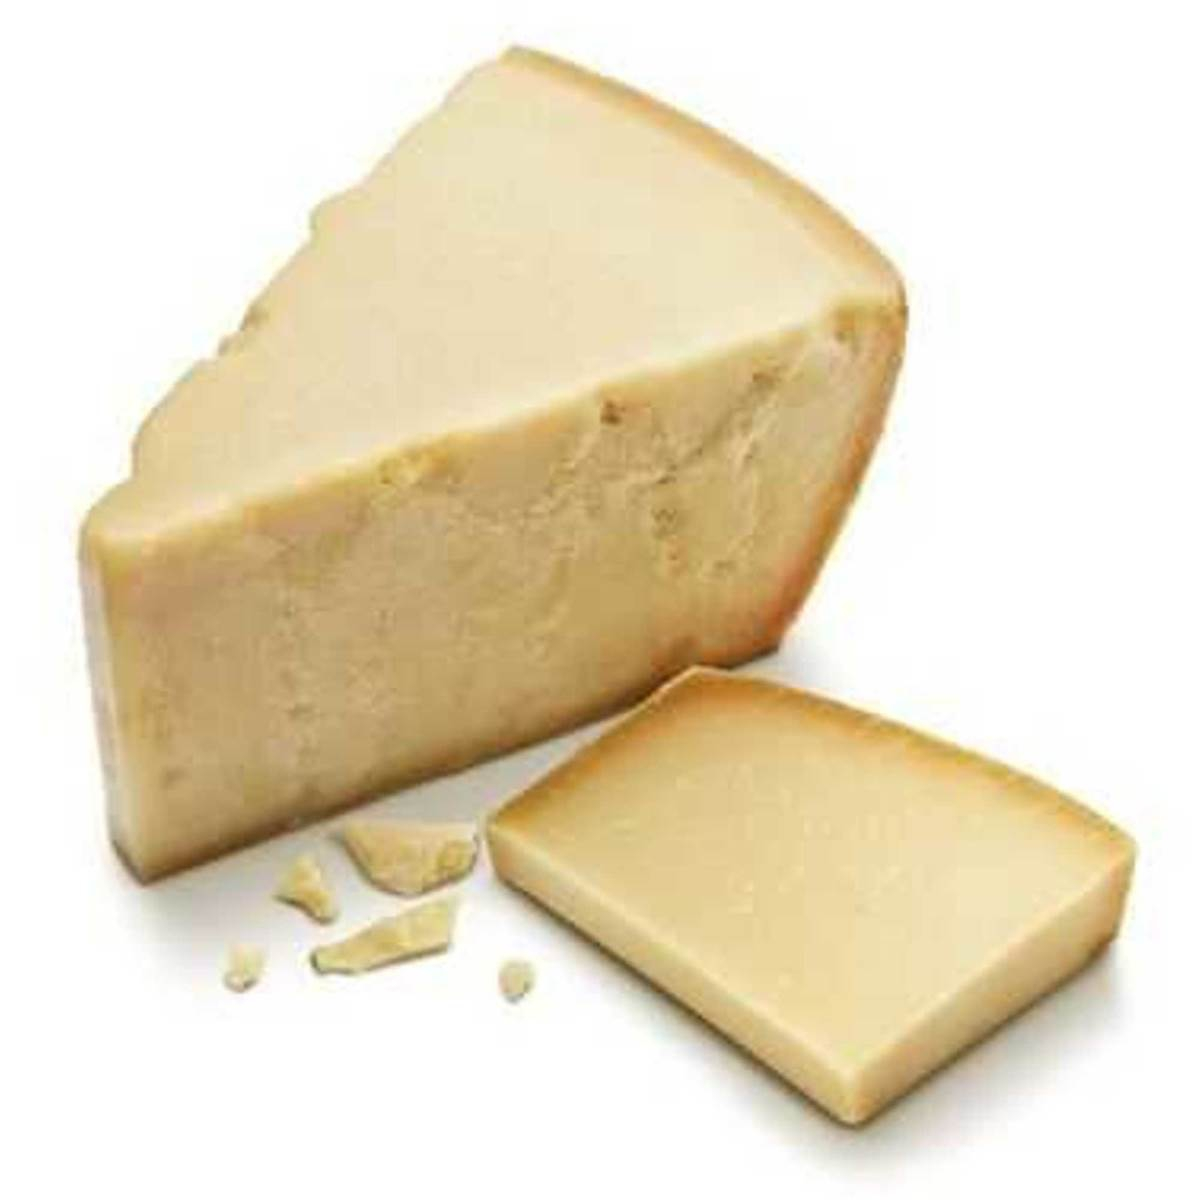
\includegraphics[width=10mm]{fig/parmezan.jpg}};
                % \draw[->,red] (bri.east) -- +(5mm,0);
                % \draw[->,red] (parm.east) -- +(5mm,0);
                % \draw[->,red] (bri.west) -- +(-5mm,0);
                % \draw[->,red] (parm.west) -- +(-5mm,0);
                \draw[->,thick] (bri.north)--(parm.south);
                % \tikz \draw (0,0) -- (0,0.6\paperheight);
            \end{tikzpicture}
            \caption*{Зависимость степени конверсии~$DC$~(a) и приведенного модуля Юнга~$E_r$~(б) от мощности лазерного излучения~$LP$. I область --- выход  на насыщение, II область --- насыщение степени конверсии и приведенного модуля Юнга.}
        \end{figure}

\end{frame}

\begin{frame}{Результаты}
        \begin{minipage}{0.60\linewidth}
            \begin{minipage}{0.49\linewidth}
                \begin{tikzpicture}
                    \node (a) {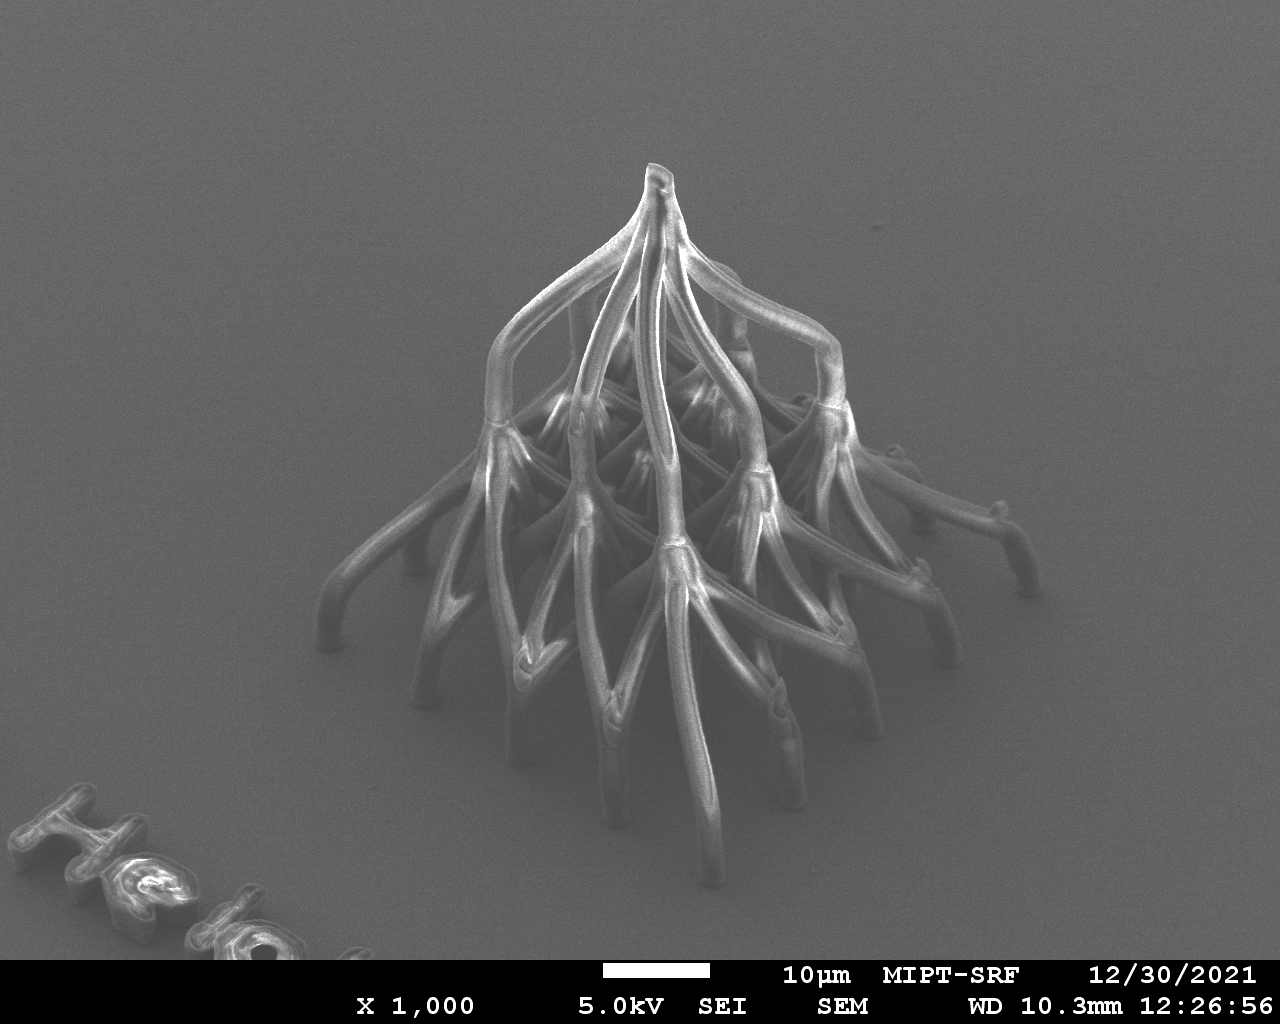
\includegraphics[width=\linewidth]{fig/t10_2.jpg}};
                \node at (a.north west)[white,xshift=4mm,yshift=-5mm] {(a)};
                \end{tikzpicture}
            \end{minipage}
            \hfill
            \begin{minipage}{0.49\linewidth}
                \begin{tikzpicture}
                \node (b){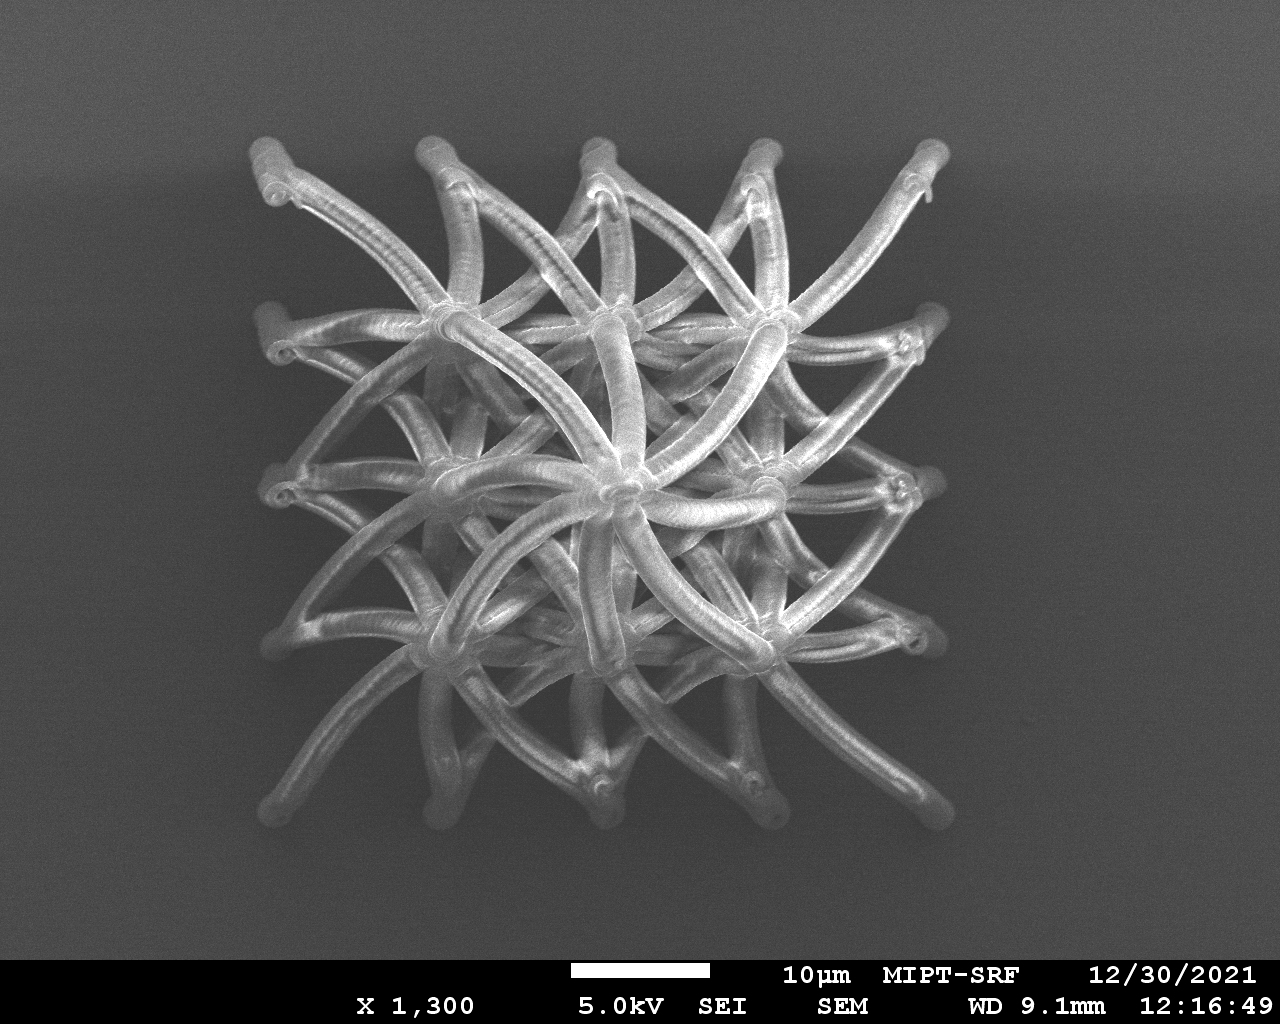
\includegraphics[width=\linewidth]{fig/t10_1.jpg}};
                \node at (b.north west)[white,xshift=4mm,yshift=-5mm]  {(б)};
                \end{tikzpicture}
            \end{minipage}
            \captionof*{figure}{(a,б)~РЭМ снимки изготовленных 3D разветвителей $1 \times 25$ входов/выходов. (в)~3D модель в DeScribe}
        \end{minipage}
        \hfill
        \begin{minipage}{0.35\linewidth}
                \begin{tikzpicture}
                    \node (model) 
                    {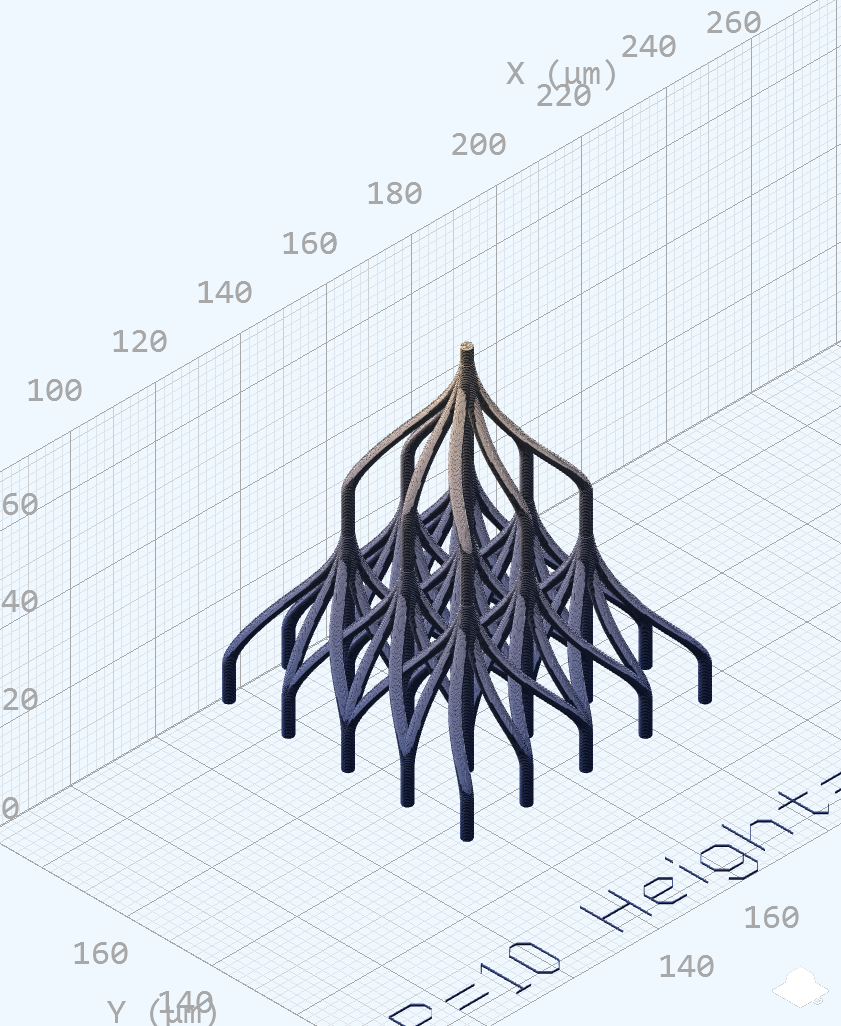
\includegraphics[width=\linewidth]{fig/Job_3x3_Mass_LP_Modify_2022-02-15_00-27-09.png}};
                    \node at (model.north west)[xshift=4mm,yshift=-2mm]  {(в)};
                    \coordinate (In_0) at (model.north);
                    \coordinate (In_1) at (model.center);
                    % \draw[->,red,ultra thick] (In_0) -- (In_1);
                    \draw[->,red,ultra thick] (2.5mm,24mm) -- +(0,-14mm) node [above=16mm] {лазер $\uplambda$};
                    % \draw[->,red,thick] (1.5mm,-10mm) -- +(0,-8mm)[xshift=3mm] (1.5mm,-10mm) -- +(0,-9mm)[xshift=3mm] (1.5mm,-10mm) -- +(0,-10mm);
                    \coordinate (Out_0) at (2.6mm,-19mm);
                    \coordinate (Out_1) at (0mm,-11mm);
                    \foreach \x in {-4,-3,...,4}{
                    \coordinate (tmp_0) at ($(Out_0) + (0.35*\x,0.05*\x*\x)$);
                    \draw[->, red, thick] (tmp_0) -- +(Out_1);
                    };
                \end{tikzpicture}
        \end{minipage}
            % \begin{minipage}{0.49\linewidth}
            %     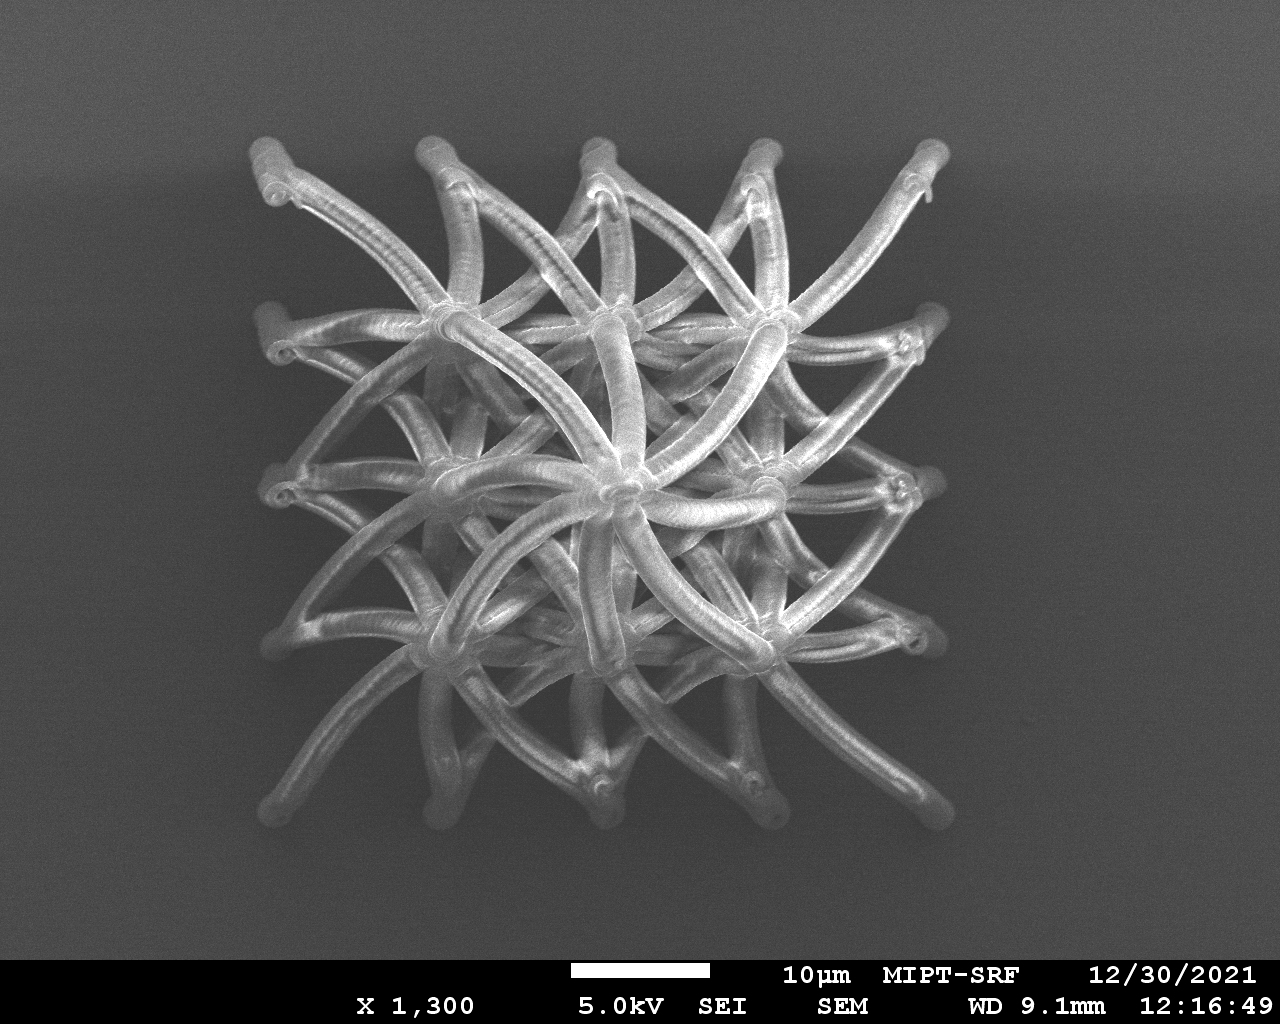
\includegraphics[width = \linewidth]{fig/t10_1.jpg}
            % \end{minipage}
            % \hfill
            % \begin{minipage}{0.49\linewidth}
            %     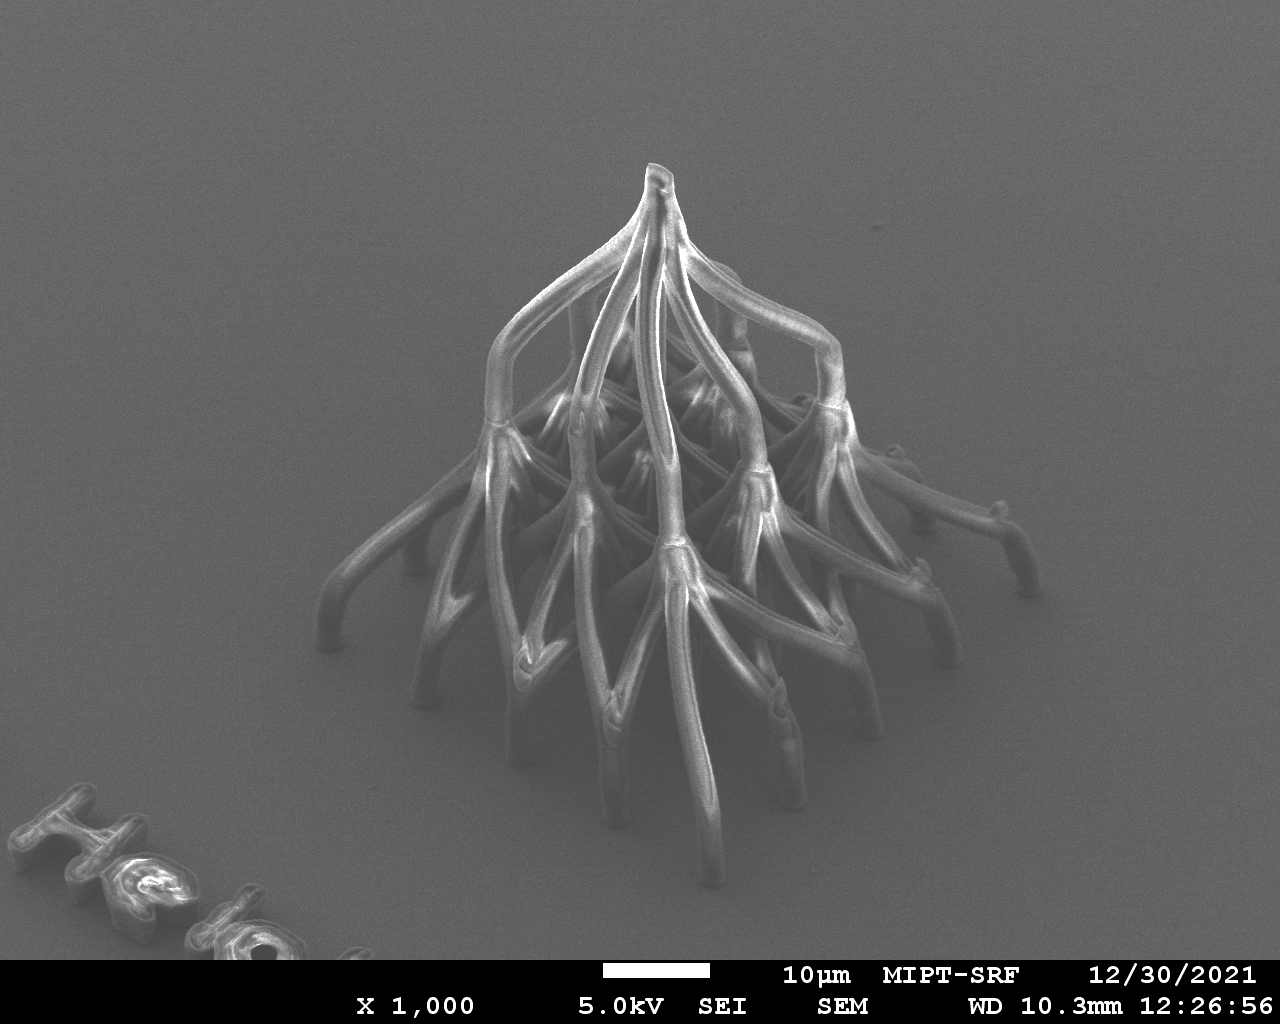
\includegraphics[width = \linewidth]{fig/t10_2.jpg}
            % \end{minipage}
            % \begin{minipage}{\linewidth}
            %     \centering
            %     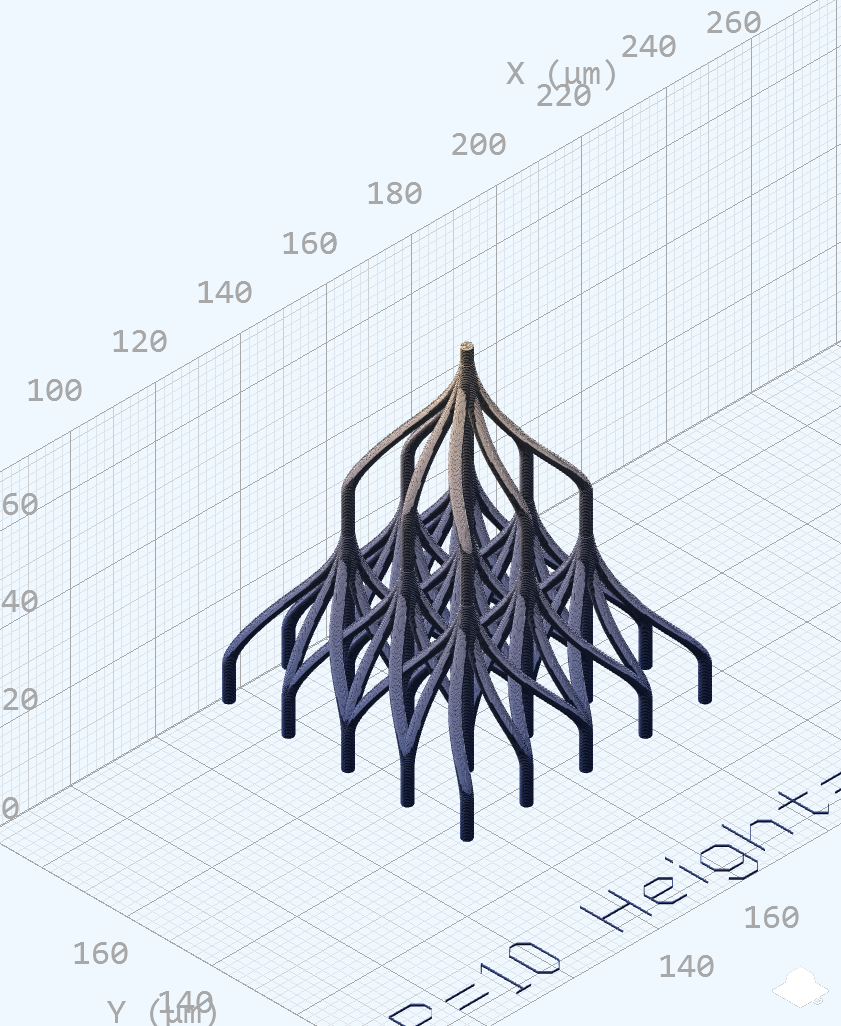
\includegraphics[width = .5\linewidth]{fig/Job_3x3_Mass_LP_Modify_2022-02-15_00-27-09.png}
            % \end{minipage}
\end{frame}

\begin{frame}{Выводы}
    \begin{enumerate}
            \item Получена зависимость размера вокселя от параметров литографии. Наблюдалось аномальное (эффект Шварцшильда) и классическое (нормальное) поведение фотокомпозиции.
            % \item Предложена и освоена методика исследования степени конверсии и модуля Юнга 3D-микроструктур. 
            \item Изучена зависимость степени конверсии и приведенного модуля Юнга от мощности лазерного излучения. Получены значения насыщения: $DC$~=~(35~$\pm$~1)~$\%$ и $E_r$~=~(1,98~$\pm$~0,15)~ГПа соответственно. Мощность излучения, с которой достигается насыщение, равна 5~мВт (при $V$ = 180 мкм/с). Это соответствует дозе $D_2$ = 3,53~мДж$^2$/мкм$^4$с.
            \item Определен оптимальный диапазон параметров DLW--нанолитографии:
            \begin{itemize}
                \item $V$ от 20~мкм/с до 80~мкм/с при мощности  $LP$~от~5~мВт до 6,5~мВт
                \item $V$ от 40~мкм/с до 60~мкм/с при мощности  $LP$~>~6,5~мВт 
            \end{itemize}
            \item Изготовлены механически устойчивые 3D-микроструктуры сложной геометрии из новой фотокомпозиции.
            \item Рассмотрены и освоены классы методик измерения: атомно-силовая микроскопия, наноиндентирование и рамановская спектроскопия.
        \end{enumerate}
\end{frame}

\begin{frame}{Публикации}
    \begin{itemize}
        \item Denis A. Shcherbakov et.al., “Morphological and Mechanical Properties of Micron- and Submicron-Scale Polymer Multi-Voxel Based on a Methacrylate-Containing Photocomposition for Two-Photon Photopolymerization”, \textit{Engineering Science and Technology, an International Journal}, \textit{under review}, 2022.
        \item Щербаков Д.А. и др., “Исследование механических свойств новой фотокомпозиции для двухфотонной 3D нанолитографии методом наноиндентирования”, \textit{Труды 64-й Всероссийской научной конференции МФТИ}, 2021.
        \item Щербаков Д.А. и др., “Исследование методом наноиндентирования 3D микроструктур, изготовленных двухфотонной нанолитографией”, \textit{14-я Международная конференция «Углерод: фундаментальные проблемы науки,материаловедение, технология»}, 2022.
    \end{itemize}
\end{frame}

\begin{frame}{Благодарности}
        \fontsize{11pt}{7.2}\selectfont
        Выражаю свою благодарность за помощь в выполнении работы:
        \begin{itemize}
            \item научному руководителю д.ф.-м.н.~Витухновскому Алексею Григорьевичу, к.ф-м.н.~Колымагину Даниле Анатольевичу к.ф.-м.н.~Чубичу Дмитрию Анатольевичу за помощь в проведении исследования, научную консультации и всестороннюю поддержку.
            \item центру коллективного пользования МФТИ и Коростылёву Евгению Владимировичу за помощь в исследовании морфологии структур методом растровой электронной микроскопией.
            \item ИМХ РАН за предоставление фотокомпозиций на основе фотоинициатора 4Met-BAC.
            \item центру коллективного пользования научным оборудованием ФГБНУ ТИСНУМ «Исследования наноструктурных, углеродных и сверхтвердых материалов», Гладких Екатерине Владимировне и Султановой Гульназ Хакимовне за помощь в проведении исследования механических свойств и использование оптического бесконтактного профилометра.
            \item Соловью Валентину Романовичу за помощь в исследовании оптических свойств методом рамановской спектроскопии.
            \item А также рецензенту к.ф.-м.н.~Токунову Юрию Матвеевичу.
        \end{itemize}
\end{frame}



% \begin{frame}[plain]
%     \miptpolygons{
%         \Huge{Спасибо за Внимание!}
%         \vfill
%     }
% \end{frame}

% \begin{frame}[noframenumbering]
% \frametitle{Приложение}
%     \large
%     Модификатор \textbf{noframenumbering} можно использовать для дополнительных слайдов в конце, чтобы они не учитывались при нумерации.
% \end{frame}


\end{document}
